%% This document gives an example on how to use the ntnumasterthesis
%% LaTeX document class.

%% Use short name MACS, MIS, CIMET, MTDMT, MIXD or MIS  
%% Language english or norsk
%% b5paper with oneside or twoside, you can set A4 if you want but you submit in b5

%% If you want print with the heading material on a4 paper you can use this format
%% \documentclass[MACS,english,a4paper,oneside,12pt]{ntnuthesis/ntnuthesis}

%% with the change to using DAIM we have a new option. include DAIM after english below removes the front page material so that you can then submit in the DAIM system. If you are wanting the front material remove DAIM and make sure you fill in the DaimData.tex file.
\documentclass[MIS,english]{ntnuthesis/ntnuthesis}

\usepackage[T1]{fontenc}
\usepackage[utf8]{inputenc}     % For utf8 encoded .tex files allows norwegian characters in the files. This can be dangerous if you change to a differnt editor.
%\usepackage[pdftex]{graphicx, hyperref}   % For cross references in pdf
\usepackage{graphicx}
\usepackage{hyperref}   % For cross references in pdf

\hypersetup{colorlinks=true,     
		linkcolor=blue,          % color of internal links (change box color with linkbordercolor)
    citecolor=blue,        % color of links to bibliography
    filecolor=blue,      % color of file links
    urlcolor=blue           % color of external links
		}
\usepackage{amsmath}
\usepackage{tikz}
\usetikzlibrary{shapes.geometric,arrows,automata}

\usepackage{pgfplots}
\pgfplotsset{width=\hsize,compat=1.15}

\usepackage{multicol}

% For smart references 
%    use \cref{label} and Caption and Number will be added automatically
\usepackage[capitalise,noabbrev]{cleveref} 

\usepackage{color}              % For colouring text 

\usepackage{csvsimple}  % for simple table reading and display
\usepackage{url}
\usepackage{booktabs}
\usepackage{gnuplottex} %miktex option if using miktex on windows
\usepackage{rotating}


\definecolor{darkgreen}{rgb}{0,0.5,0}
\definecolor{darkred}{rgb}{0.5,0.0,0}

\lstset{        basicstyle=\ttfamily,
                keywordstyle=\color{blue}\ttfamily,
                stringstyle=\color{darkred}\ttfamily,
                commentstyle=\color{darkgreen}\ttfamily,
}

%Typesetting of C++ but not always stable in titles etc...
\newcommand{\CPP}[0]{{C\nolinebreak[4]\hspace{-.1em}\raisebox{.1ex}{\small\bf +\hspace{-.1em}+\ }}}

%\usepackage[table]{xcolor}% http://ctan.org/pkg/xcolor
%\usepackage[nomessages]{fp}
%\newlength{\maxbarlen}


\newcommand\databar[3][gray!20]{%
  \FPeval\result{round(#3/#2:4)}%
  \rlap{\textcolor{#1}{\hspace*{\dimexpr-\tabcolsep+.5\arrayrulewidth}%
        \rule[-.05\ht\strutbox]{\result\maxbarlen}{.95\ht\strutbox}}}%
  \makebox[\dimexpr\maxbarlen-2\tabcolsep+\arrayrulewidth][r]{#3}}



\newcommand{\com}[1]{{\color{red}#1}} % supervisor comment
%\renewcommand{\com}[1]{} %remove starting % to remove supervisor comments
% This will appear in text \com{Lecuters comment} and be visible unless you uncomment
% the renewcommand line.

\newcommand{\todo}[1]{{\color{green}#1}} % items to do
%\renewcommand{\todo}[1]{} %remove starting % to remove items to do

\newcommand{\n}[1]{{\color{blue}#1}} % other comment
%\renewcommand{\n}[1]{} %remove starting % to remove notes


\newcommand{\nikolai}[1]{{\color{orange}#1}} % other comment
\newcommand{\anders}[1]{{\color{purple}#1}} % other comment
%\renewcommand{\n}[1]{} %remove starting % to remove notes

\newcommand{\dn}[1]{} % add the d to a note to say that you have finished with it.





% Set to true ONLY if using Harvard citation style
\newboolean{HarvardCitations}
\setboolean{HarvardCitations}{false} % false for computer science, true for interaction design and harvard style


\ifthenelse{\boolean{HarvardCitations}}{%
	\usepackage{natbib} % for Harvard names as citations.
}{%
	\usepackage[numbers]{natbib} % for Vancover numbers in bibliography
}

\newcommand{\q}[1]{\leavevmode\marginpar{\small\em #1}}
\renewcommand{\q}[1]{}


\begin{document}

% for students submitting in the DAIM system this information will not be used.
% their is an option for DAIM submission which removes this information and checks it is B5.
% Removing the DAIM option on the document type will use this material.

\setthesistitle{Real Time Windows Event Log Analysis}
\setthesisshorttitle{Real Time Windows Event Log Analysis} % a short version for the page headers if your normal title is too long to fit
\setthesisauthor{Martin Ingesen}
\setthesissupervisor{Ass. Prof. Geir Olav Dyrkolbotn}
%\setthesissupervisorA{Prof. ?}  % if you have a second supervisor add it like this
%\setthesissupervisorB{Prof. Smart Guy}  % if you have a second supervisor add it like this


\nmtkeywords{Thesis, Latex, Template, IMT}
%\nmtdesc{This is the short description of a masters thesis}


\setthesisdate{02-06-2020}
\setthesisyear{2020}



%for CIMET theses you need to see all of these as well

%\setthesiscampus{Gj\o{}vik}
%\setthesisHostInstitution{\NTNU}
%\setthesisHostInstitution{University of Eastern Finland}
%\setthesisHostInstitution{Universit\'e Jean Monnet Saint-Etienne}

%\setthesisjuryA{} %jury names
%\setthesisjuryB{} %jury names
%\setthesisjuryC{} %jury names
%\setthesisjuryD{} %jury names


 % this is the file which contains all the details about your thesis
\makefrontpages % make the frontpages
%\thesistitlepage % make the ordinary titlepage
\hypersetup{pageanchor=false}
%\include{summary}

\chapter*{Preface}
The following thesis deals with rule-based event correlation alerting in real time, based on Windows Event Log. This is a a Master's thesis in MIS (Master in Information Security) at NTNU Gjøvik, carried out during the spring semester in 2020. The idea for the thesis was brought up during my work at BDO AS, where their CERT was exploring the same issue with creating high fidelity alerts from Windows Event Log in a real-time fashion.

The thesis is targeted at audience from the field of information technology and especially those working with security monitoring. However, no expert knowledge is required as the thesis explain all terms and methods used.\\[2cm]
\iffalse
The following work deals with multinomial malware classification of ten malware families with machine learning algorithms. It is carried out in the context of a Master’s thesis in MIS (Information
Security) at NTNU. It was conducted during the spring semester 2019. The broad idea of the topic
was brought up by my supervisors before it was specified in more detail and finalised in a direct
discussion between us. It is still a relevant topic today since the malware landscape is constantly
growing and evolving and therefore, further research has to be conducted in the area of this topic.
Nonetheless, the thesis is targeted at an audience from the field of information technology with the
focus on forensics. However, no expert knowledge of the malware landscape is needed to understand the elaboration since all used terms and methods are explained.

Here, you give a brief introduction to your work. What it is (e.g., a Master's thesis in AIMT at NTNU, when it was carried out (e.g., during the autumn semester of 2021). If the project has been carried out with a company, you should mention this and also describe the cooperation with the company. You may also describe how the idea to the project was brought up.

You should also specify the assumed background of the readers of this report (who are you writing for).\\[2cm]
\fi
%\begin{center}
%\thesiscampus, 
\thesisdate \\[1pc]
\\[1pc]
%\thesisauthor
%\end{center}

\chapter*{Acknowledgment}
Foremost, I would like to express my sincere gratitude to my supervisor, Ass. Prof. Geir Olav Dyrkolbotn for providing excellent guidance, assistance and support during this thesis. I especially appreciate how my supervisor has facilitated guidance from me as a distance student at NTNU.

A big thank goes to my employer BDO AS, and especially Ingunn Holte and Håkon Lønmo, for allowing me time to research, study and write my thesis while working full-time.

I highly appreciate all motivation and support from friends and family throughout my studies. I especially couldn't have done this without my partner Cecilie which has supported me through all ups and downs along the way. I would also like to mention our son Arthur who never failed to cheer me up when I was stuck or met an obstacle during my writing of this thesis.

\begin{flushright}
M.I.\\[1pc]
\end{flushright}

\chapter*{Abstract}
\iffalse
LES "Scrutiny of the abstract" referert i Scrutiny of the introduction - http://sepwww.stanford.edu/sep/prof/Intro.html
\fi
This is a summary of the thesis including the conclusion of what was discovered.

\chapter*{Sammendrag}
\iffalse
LES "Scrutiny of the abstract" referert i Scrutiny of the introduction - http://sepwww.stanford.edu/sep/prof/Intro.html
\fi
Dette er et sammendrag...

\hypersetup{pageanchor=false}

\tableofcontents

\hypersetup{pageanchor=true}

% Comment with a percent to remove figures or tables:
\listoffigures
\listoftables
\lstlistoflistings

% ======== INSERT STUFF HERE vvv ========
\chapter{Introduction}
\label{chap:introduction}

\iffalse
Scrutiny of the introduction - http://sepwww.stanford.edu/sep/prof/Intro.html
\fi

%Why do we need to monitor?
New vulnerabilities and attack vectors are discovered every day. Cyber attacks can critically impact and cripple businesses that are targeted. Many of these cyber threats focus on penetrating the network of a business to steal valuable information, hold data as ransom or permanently destroy the business network. The cost of a cyber attack can be high, and is not only measured in lost data or equipment, but also the business reputation and client-base. This is why it is important to identify such attacks as soon as possible.
%What has traditionally been the way we monitor?
Traditionally, network security monitoring (NSM) has been essential to avert these cyber threats and attacks. 
NSM is the collection, analysis, and escalation of indications and warnings to detect and respond to intrusions in the network. The goal is to detect and respond to threats as early as possible to prevent unauthorized access, misuse, destruction or data theft.
%What methods are commonly used in monitoring?
The most common way to do network security monitoring, is to use solutions known as "Intrusion Detection Systems" (IDS) or "Intrusion Prevention Systems" (IPS). These systems are used to detect, alert and possibly prevent security incidents from occurring by monitoring the network traffic that flows to and from the computers in the business network, and out to the internet. The main benefits of using these network-based solutions, is that there is no need to alter the existing infrastructure or install any software on the hosts in the network. The solutions monitor everything on the network segment they are placed in, regardless of the operating systems (OS) running on the hosts. An additional factor has been the fact that these solutions have a lower cost of setup and maintenance than host-based solutions that require installing or configuring software on the hosts themselves.
%What are the weaknesses with these methods?
But as businesses are moving to become more and more digital, and the workforce is getting accustomed to working from anywhere, be it from home, from the coffee shop or even from the beach, the business network-perimeter is slowly being eroded away.
As of writing this, the COVID-19 virus is spreading across the globe, and employees all around the world are forced to stay at home to reduce the risk of spreading the disease. This global pandemic is forcing those businesses who have not already adapted to a remote workforce, to introduce work-from-home quickly.
In addition to the work-from-home factor, we are also seeing a rise in encrypted traffic, both between hosts, but also out to the wider internet. Privacy-enhancing technologies like DNS-over-TLS/DNS-over-HTTPS, free TLS certificates and browsers marking unencrypted websites as "unsafe" are pushing the bar on moving to a fully-encrypted internet. Unless the business chooses to utilize TLS interception to "see" the encrypted traffic inline using their traditional network security monitoring solutions, they are increasingly becoming blind to the threats that might hide behind encrypted communications. There is also no visibility into what is actually happening on the hosts in the network, unless there is data transmitted across the network that can be analyzed. All of these factors contribute to a reduced value in network-based security monitoring.
%What is the solution to this?
The industry solution to this has been to shift focus away from network-based monitoring and detection, and take a more endpoint-centric approach.
First of all we have host-based intrusion detection systems (HIDS) which monitor the dynamic state of the host, and alerts on system changes that are out-of-place. This is usually based on a database containing the cryptographic hash of known-good files. The HIDS then monitor the files for any changes, and report any changes to a central location. Then we have the common anti-virus/anti-malware/endpoint protection software. These software solutions usually contain a range of different detection and prevention methods, and usually incorporates a variety of signature-based, heuristic-based, data mining and machine learning detection. Commercial-grade anti-virus (AV) usually reports their findings to a central location for analysis. Lastly, we have event forwarding, which is software that sends the events generated by the OS to a central location for detection, analysis and forensic purposes. Storing all the logs, not just alerts like anti-virus and HIDS might do, in a central location has the added benefit of being able to be searched in after-the-fact. This makes event forwarding very valuable for forensic purposes and for developing new detections based on historical data.
%What are the drawbacks?
Historically, there has been concerns with all of these solutions. The different solutions have in general been hard to install, configure and maintain on the individual hosts in a business, and the alerts produced by the anti-virus or HIDS has to be transmitted and stored in a central location. In addition, performance degradation on the hosts caused by the resource-intensive software required for detection, prevention and transmitting alerts has been of concern.
For anti-virus to protect its integrity and detect malice it has to run with high privileges on the host. Any vulnerabilities in the AV engine can then have fatal consequences allowing for instance privilege escalation on the host. There has been concerns regarding system instability caused by bugs in the AV engine or slow network connections caused by the AV doing network inspection. These faults are usually patched or corrected quickly by the vendor, but might still be of concern to the system administrators. Event forwarding requires knowledge of what logs to forward and what to filter out. The number of events that are generated per second can vary, and being able to estimate the amount of logs are important so that the central log collection can be scaled appropriately to accommodate the volume of logs that are being ingested and stored.
In recent years, the technology both for configuring and maintaining software on the hosts and systems for ingesting host data to a central location has done great leaps. Vendors of security products have made their software simpler to configure, usually via a cloud-based console. Storage is in general cheaper, and "Security Information Event Management" (SIEM) software has made it simpler to monitor and analyze large volumes of event and log data.

\section{Problem description}
\label{sec:problemdescription}

\todo{This is not done}

One of the remaining problems with event forwarding, is the ability to search, 

being able to write rules that are able to correlate in real time against event log data in real time.

Current detection analysis is based on aggregating log files into a centralized system known as a System Information and Event Management (SIEM) system. Traditionally in a SIEM, logs are analyzed after-the-fact. This has several drawbacks as this type of security monitoring is reactive and requires actively hunting for bad events in the data using dashboards or search queries that are executed by the analyst.
Another huge problem with pure SIEM-based logging, as companies are collecting more and more logs, actively hunting for badness in those logs are becoming harder and more complex. I single log item from a single source is not enough to properly analyze what has happened in a system. Only by cross-correlating several log lines and log sources are we able fully understand the situation at hand and create detection that are of high quality.

\section{Justification, motivation and benefits}
\label{sec:motivation}
Today, event log correlation is usually done using built-in functionality in a SIEM, or specialized software that processes data.
There is a big demand for solutions that are able to correlate large amounts of event log in real time....

%What are the drawbacks?
Host-based logging can produce huge amounts of events.
Being distributed, not everyone are sending their event logs at the same time. There will be delays, and events may appear in the "wrong" order. Eg. not sequential.

Popular SIEM solutions are mostly commercial and costly.
%What are the benefits with such a system?
There are several benefits to a system like this.

Allows analysts to write rules that can be added to the rule repository and instantly be used. Does not require any configuration changes, software deployments or system restarts.

% What do we contribute?
In this thesis we contribute an improved method for correlating Windows Event Logs in real-time, while at the same time taking care to address the problems with log ingestion delays and asynchronous events.

\section{Research questions}
\label{sec:researchquestions}
To solve the problems outlined in \ref{sec:problemdescription}, the following research questions have been developed:\\\\
\textbf{Hypothesis:} We believe that we are able to improve upon current research and methods for real time event correlation, by utilizing a compiled, multi-threaded programming language and better rule formats.\\
\textbf{Research questions:}
\begin{enumerate}
    \item What is the state of the art for real time event correlation?
    \item How can we improve the way real time event correlation is done for Windows Event Logs? %How can multi-threaded programming language and netter rule formats improve how real time event...
    \item What is the performance of our proposed method, and how does it compare to other methods?
\end{enumerate}

\section{Planned contributions}
\label{sec:plannedcontributions}

The primary contribution of this project is an improved method for correlating Windows Event Logs in time, in near real time. The goal of this thesis is to explore ways to improve real time log correlation both performance-wise but also addressing the problems that occur when analyzing asynchronous events or when experiencing log ingestion delays.

\section{Thesis outline}
\label{sec:thesisoutline}
This section presents an overview of the thesis and a short summary of each chapter.\\\\
\textit{Chapter X: A}\\
\n{This is some text}\\\\
\textit{Chapter Y: A}\\
\n{This is some text}
\chapter{Related Work}
\label{chap:relatedwork}


\chapter{Background}
\label{chap:background}

In this chapter...

\section{Event correlation}

\subsection{Scenario-based Correlation}
\iffalse
https://dl.acm.org/doi/pdf/10.1145/1501434.1501479
\fi
\subsection{Statistical Correlation}
\subsection{Temporal Correlation}
\subsection{Hybrid approaches}

\iffalse
\cite{Ludovic_2004} to propose a fully functional intrusion detection system based on event and alert correlations. Among the several approaches available in the literature, we chose to implement a language driven signature based correlation. Uses FSM to implement the multi-pattern rule matching detection algorithm.
\fi
\subsection{Finite State Machine Based}
% What are finite state machines?
A finite-state machine, a system is abstracted into mathematical model which can have exactly one of a finite number of states at a time. A finite-state machine has a fixed set of possible states, a set of inputs that change the state, and a set of possible outputs \cite{keller_2001}.
The next state of a finite-state machine is based on the current state that the machine is in, and the input that change the state.
There are generally considered to be two kinds of finite-state machines, deterministic finite-state machines and non-deterministic finite-state machines. In a deterministic finite-state machine, every state has only one transition per input, as opposed to the non-deterministic state machine, where an input can lead to none, one or many transitions for a given state. Since the deterministic finite-state machine is a more strict version of the non-deterministic finite-state machine, that leads to that by definition, a deterministic finite-state machine is also a non-deterministic finite-state machine.
For example, assuming that we have the following three events in order:
\begin{enumerate}
    \item the process '$word.exe$' started
    \item the process '$googlechrome.exe$' started
    \item The process '$powershell.exe$' started
\end{enumerate}
If we want to trigger an alert when we see the $word.exe$ process is created, and then the $powershell.exe$ process afterwards, we can design a simple non-deterministic state machine like the one in figure \ref{fig:finite-state-machine}. When applying the above-mentioned events to this finite state-machine, event number one will move our state from $s_0$ to $s_1$. Event number two will not do any transitions and change the state (one of the benefits of using a non-deterministic state machine). When event number three occurs, the state machine transitions from $s_1$ to $s_2$, and our accepting state is reached, which fulfills the state machine and we can create an alarm.
\begin{figure}[ht]
\centering
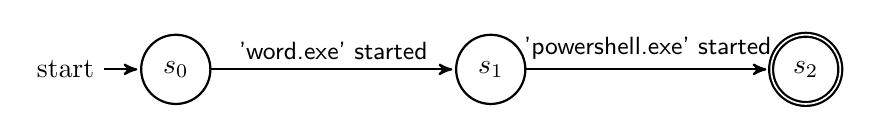
\begin{tikzpicture}[->,>=stealth',shorten >=1pt,auto,node distance=4cm,
                    thick,main node/.style={circle,draw,font=\sffamily\Large\bfseries}]
  \node[initial,state] (p1) {$s_0$};
  \node[state] (p2) [right of=p1] {$s_1$};
  \node[state,accepting] (p3) [right of=p2] {$s_2$};

  \path[every node/.style={font=\sffamily\small}]
    (p1)
        edge node {'word.exe' started} (p2)
    (p2)
        edge node {'powershell.exe' started} (p3)
    ;
\end{tikzpicture}
\caption{Example of non-deterministic finite-state machine}
\label{fig:finite-state-machine}
\end{figure}
One of the benefits of the finite-state model is that it is possible to specify if the order of the events are important or not. If the event order is not of interested, a finite-state machine as shown in Figure \ref{fig:finite-state-machine-2} can represent the same case as seen in Figure \ref{fig:finite-state-machine}.
\begin{figure}[ht]
\centering
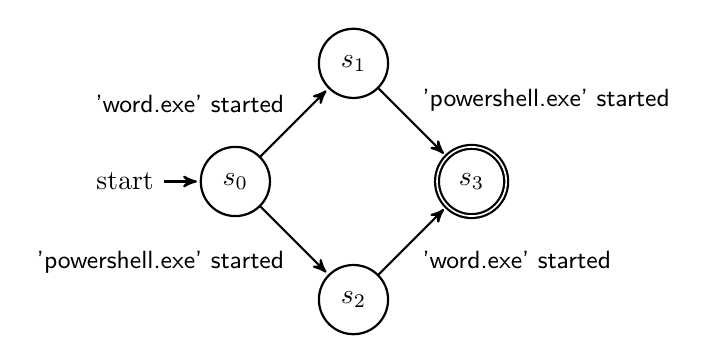
\begin{tikzpicture}[->,>=stealth',shorten >=1pt,auto,node distance=1.5cm,
                    thick,main node/.style={circle,draw,font=\sffamily\Large\bfseries}]
  \node[initial,state] (s0) {$s_0$};
  \node[] (middle) [right of=s0] {};
  \node[state] (s1) [above of=middle] {$s_1$};
  \node[state] (s2) [below of=middle] {$s_2$};
  \node[state,accepting] (s3) [right of=middle] {$s_3$};

  \path[every node/.style={font=\sffamily\small}]
    (s0)
        edge node {'word.exe' started} (s1)
        edge node [swap] {'powershell.exe' started} (s2)
    (s1)
        edge node {'powershell.exe' started} (s3)
    (s2)
        edge node [swap] {'word.exe' started} (s3)
    ;
\end{tikzpicture}
\caption{Example of non-deterministic finite-state machine}
\label{fig:finite-state-machine-2}
\end{figure}

An approach to use finite-state machines for event correlation has been shown in \cite{Bouloutas_1992} where the authors use observed events that are generated by the monitored process to feed into the modelled finite-state machine that represent the monitored process. If an event arrives that leads to an invalid state in the model, an error is produced.

One of the main drawback with the finite-state machine is the missing notion of time. As shown in Figure \ref{fig:finite-state-machine-2} we can take into account order of events, but a finite-state machine does not separate on the time difference between events that are streamed into the model.

\subsection{Rule Based Event Correlation}
\subsection{Case Based Reasoning}

In case based reasoning, a previously experienced problem and its solution is called a case. As explained in \cite{aamodt_1994}, case based reasoning is based on the assumption that we can find a solution for a new problem by finding past cases that are similar, and then reusing the solution to solve the new problem. The reasoning is then further enforced by adding the problem and the solution to the case library for future use.
As stated in \cite{slade_1991}, case-based reasoning is similar to how humans approach new problems by assimilating past experiences and adapting them to new situations.

Figure \ref{fig:case-based-reasoning-cycle} describes the cycle used in case-based reasoning from a high-level perspective.
Under each step in the cycle there are multiple tasks that may be necessary to conduct before continuing on with the cycle. For instance, the "Retrieve" step might need to identify which features of the problem to search the Case Library for.
\begin{figure}[ht]
\centering
%\tikzstyle{startstop} = [rectangle, rounded corners, minimum width=3cm, minimum height=1cm,text centered, draw=black, fill=red!30]
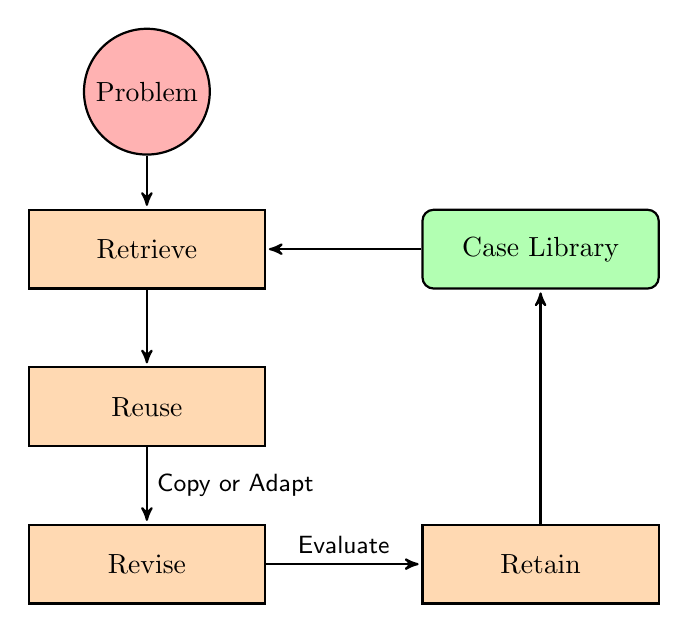
\begin{tikzpicture}[->,>=stealth',shorten >=1pt,auto,node distance=2cm,
                    thick,main node/.style={circle,draw,font=\sffamily\Large\bfseries},
                    problemm/.style={circle, text centered, draw=black, fill=red!30},
                    stepp/.style={rectangle, minimum width=3cm, minimum height=1cm,text centered, draw=black, fill=orange!30},
                    libraryy/.style={rectangle, rounded corners, minimum width=3cm, minimum height=1cm,text centered, draw=black, fill=green!30}]
  \node (Problem) [problemm] {Problem};
  \node (Retrieve) [stepp, below of=Problem] {Retrieve};
  \node (Reuse) [stepp, below of=Retrieve] {Reuse};
  \node (Revise) [stepp, below of=Reuse] {Revise};
  \node (Retain) [stepp, right of=Revise, xshift=3cm] {Retain};
  \node (CaseLibrary) [libraryy, right of=Retrieve, xshift=3cm] {Case Library};
  
  \path[every node/.style={font=\sffamily\small}]
    (Problem)
        edge node {} (Retrieve)
    (Retrieve)
        edge node {} (Reuse)
    (Reuse)
        edge node {Copy or Adapt} (Revise)
    (Revise)
        edge node {Evaluate} (Retain)
    (Retain)
        edge node {} (CaseLibrary)
    (CaseLibrary)
        edge node {} (Retrieve)
    ;
\end{tikzpicture}
\caption{Case-based reasoning cycle}
\label{fig:case-based-reasoning-cycle}
\end{figure}\\
A example where this might be useful is in a Security Operations Center (SOC). A SOC receives a high number of alerts that have to be handled by an analyst to analyse and propose a response to the alert. The response can vary from simply suppressing the alert as a false-positive, sending an e-mail to the client to alert them, or escalating the alarm to the Incident Response team. Case based reasoning can then be applied to new alerts by first retrieving the most similar alerts previously handled. The information stored in the previous case can then be used to handle the analysis or solution to an alert. The analyst will then revise the proposed solution, and retain the parts that might be useful for resolving similar future alerts. This follows the case based reasoning cycle proposed in \cite{aamodt_1994}.
The retrieval step is difficult because we need to find similar cases that offer solutions that are relevant. Cases may contain attributes that are irrelevant, which might not be clear to the automated retrieval process. \cite{lewis_1993} and \cite{davies_1987} propose creating "determination rules" or "determinators" that are either compound attributes or a pointer to which attributes to look at in the case.
Additionally, adaptation of the old solutions to the new problem is a difficult task. While manual specification of the solution in the "Revise" step is possible and somewhat required, too much emphasis on manual intervention or adjustments will defeat the purpose of case-based reasoning. This is why according to \cite{leake_1996} many case-based reasoning systems have adapted the cycle from Retrieve-Reuse-Revise-Retain to a much shorter Retrieve-Propose cycle that completely eliminates the adaptation.

In \cite{schwartz_2002}, the authors used the intrusion detection system Snort as a basis for a new case-based reasoning IDS that uses the Snort rule base as a case library. Snort rules may in general be too specific and fail to detect certain kind of intrusions, but with the case-based reasoning approach, the retrieval step in the cycle will take care of this by finding cases (rules) that are applicable to the network packet even though the vanilla rule would not create an alert on that packet.
In \cite{Kapetanakis_2014}, the authors argue that with the digital traces left by an attacker, it is possible to build a profile for that attacker which can be used to assist in future attacks to identify which attacker is attacking. In \cite{han_2016} the authors implemented a system called "WHAP" which uses case-based reasoning to compare cyber attacks against websites. WHAP builds on a large database of website defacements, which are custom webpages left on the victim server by the attacker to claim credit for a website hack. The system is then able to take new hacked websites as input, and output similar previous cases where it is likely that the website has been hacked by the same attacker. This can be useful for attribution and forensic investigations.

\subsection{Model Based Reasoning}
Model-based reasoning is a expert system where the target is to create a model that can be used to predict the outcome of input event or faults in the system. The idea of modelling the structure and behavior of a system has its roots in \cite{davies_1987} where their work explore the use of such models in troubleshooting digital electronics.  There are no fixed way for how a system can or should be modelled. The model itself can be created as a logical formalization using pure mathematics, or as a simulated system using for example a game engine. As the authors of \cite{Dodig-Crnkovic2017} highlight, there is an increased interest in automating the creation of the model of a system. This is based on the fact that creating and keeping a model consistent with the system it is supposed to model, is hard.
In \cite{jakobson_1993} model-based reasoning is discussed for alarm correlation for fault management in telecommunications networks.


\iffalse


The managed system is modeled
with respect to its event emission behavior (event model). The programmed knowledge somehow
defines events to be related under some temporal or sequential constraints

A description of the 


structure, the topology, connectivity of components
behaviour description,
a set of principles to guide the troubleshooting \cite{davies_1987}

\fi

In the paper \cite{poll_2003}, a figure similar to \ref{fig:model-based-reasoning-example} is shown. It outlines the process for checking if a modelled system is consistent with the real world system it is supposed to replicate.

\begin{figure}[ht]
\centering
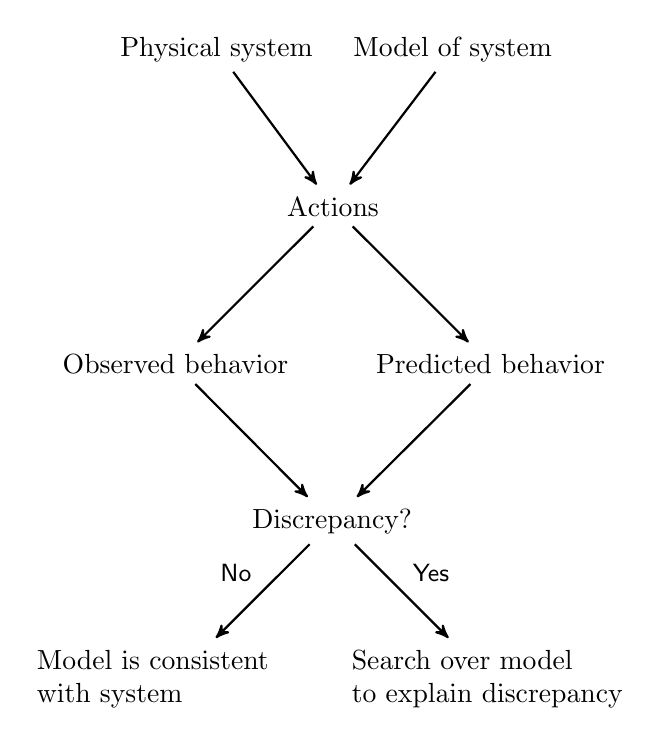
\begin{tikzpicture}[->,>=stealth',shorten >=1pt,auto,node distance=2cm,thick
                    ]
  \node (PhysicalSystem) [xshift=-1cm] {Physical system};
  \node (Model) [xshift=1cm, right of=PhysicalSystem] {Model of system};
  \path (PhysicalSystem) -- (Model) coordinate[midway] (aux);
  
  \node (Actions) [below of= aux] {Actions};
  
  \node (Observed) [below of= Actions,xshift=-2cm] {Observed behavior};
  \node (Predicted) [below of= Actions,xshift=2cm] {Predicted behavior};
  \path (Observed) -- (Predicted) coordinate[midway] (aux2);
  
  \node (Discrepancy) [below of= aux2] {Discrepancy?};
  
  \node (no) [below of= Discrepancy,xshift=-2cm,text width=3.5cm] {Model is consistent with system};
  \node (yes) [below of= Discrepancy,xshift=2cm,text width=3.5cm] {Search over model\\to explain discrepancy};
  
  \path[every node/.style={font=\sffamily\small}]
    (PhysicalSystem)
        edge node {} (Actions)
    (Model)
        edge node {} (Actions)
    (Actions)
        edge node {} (Observed)
        edge node {} (Predicted)
    (Observed)
        edge node {} (Discrepancy)
    (Predicted)
        edge node {} (Discrepancy)
    (Discrepancy)
        edge node [swap] {No} (no)
        edge node {Yes} (yes)
    ;
\end{tikzpicture}
\caption{Illustration of model-based reasoning}
\label{fig:model-based-reasoning-example}
\end{figure}
As stated in \cite{sethi_2001}, one of the primary drawbacks of model-based reasoning is the requirement to have a well structured system to model and to keep that model updated. Systems that contain fluctuating objects like for example computer networks or network services are not trivial to represent in a formal model. More applicable areas might include hardware diagnostics like shown in \cite{davies_1987}, or other areas where it is possible to model a more static target system, like for example automobile diagnostics. Furthermore, \cite{Venkatasubramanian_2003} discuss that various implementations of model-based reasoning is quite computational complex, depending on number of objects in the model and their various inputs and outputs.

\subsection{Codebook Based Event Correlation}
\label{sub:codebook-based-event-correlation}

\begin{figure}[ht]
\centering
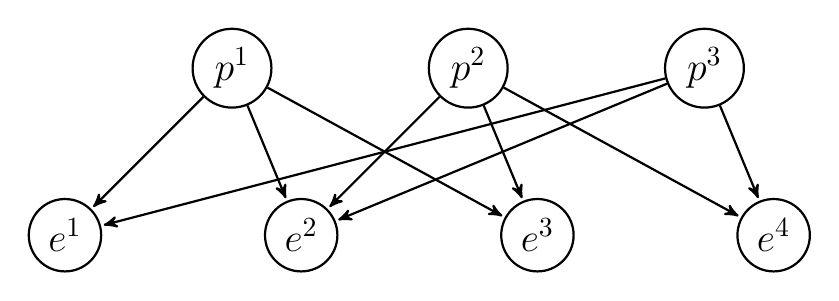
\begin{tikzpicture}[->,>=stealth',shorten >=1pt,auto,node distance=3cm,
                    thick,main node/.style={circle,draw,font=\sffamily\Large\bfseries}]
  \node[main node] (p1) {$p^1$};
  \node[main node] (p2) [right of=p1] {$p^2$};
  \node[main node] (p3) [right of=p2] {$p^3$};
  \node[main node] (e1) [below left of=p1] {$e^1$};
  \node[main node] (e2) [right of=e1] {$e^2$};
  \node[main node] (e3) [right of=e2] {$e^3$};
  \node[main node] (e4) [right of=e3] {$e^4$};

  \path[every node/.style={font=\sffamily\small}]
    (p1)
        edge node {} (e1)
        edge node {} (e2)
        edge node {} (e3)
    (p2)
        edge node {} (e2)
        edge node {} (e3)
        edge node {} (e4)
    (p3)
        edge node {} (e1)
        edge node {} (e2)
        edge node {} (e4)
    ;
\end{tikzpicture}
\caption{Example causality graph used for codebook based event correlation}
\label{fig:causality-graph-codebook}
\end{figure}

In \cite{yemini_1996}, the authors propose that the events caused by problems can be modelled as seen in figure \ref{fig:causality-graph-codebook} where the directed edges of the graph describe the causality of an event. $p^x$ denotes a problem, and $e^x$ denotes an event. To utilize the codebook, each problem node in the graph is converted into a binary vector can be created to describe its relation to the events on the graph. This is known as a "code". The binary vector contains bits that corresponds to each event in the graph. If a bit is set to a $1$, it indicates that the given problem causes the event that the bit corresponds to. A bit of $0$ indicates that it does not cause the event. These codes then go into the codebook. If we convert the graph in figure \ref{fig:causality-graph-codebook} into a codebook, it will look like table \ref{tab:correlation-matrix}. The graph and codebook needs to be sufficiently large to be able to identify all the problems. If the codebook is too small, it may omit events that are of interest to us. If the codebook is too large, it may contain events that are unnecessarily redundant. One way to approach the problem with codebooks that are too large, is to do what the authors in \cite{yemini_1996} calls "codebook reduction". Codebook reduction is the process of removing events that are "universal" for all problems. In the figure \ref{fig:causality-graph-codebook} and the corresponding table \ref{tab:correlation-matrix} we can see that event $e^2$ is a common event for all the problems. Because of this redundancy, it can be remove to simplify the codebook as show in table \ref{tab:correlation-matrix-reduced}. Further work has been done to enhance the efficiency of the codebook. \cite{gupta_1999} proposes a two step preprocessing algorithm that ensures mathematical provable codebooks and eliminates events that are unable to distinguish between problems.

When new events occur, the events are converted into a new binary vector. This vector is then compared with the codes in the codebook, and the code that is the most similar is chosen as a means to identify the problem. A simple approach for comparing the binary vectors could be a 1-to-1 comparison to see if the new binary vector exactly matches any of the codes in the codebook, but \cite{yemini_1996} propose to instead use Hamming distance to calculate the closest match. Using Hamming distance has several benefits, first of all it increases the tolerance for noise or lost events, secondly instead of choosing a single best candidate problem, we can defined a radius that will give us a codebook subset containing possible codes within the given Hamming distance radius.
Because of the novel preprocessing down to binary vectors, codebook-based correlation is faster than other rule-based event correlation techniques. One of the more time-consuming tasks with regard to codebook-based event correlation is the creation of the problems and their mapping to symptom events. The most likely way to produce these codebooks will be as an expert system where a person with deep knowledge about the events in the system are able to map symptoms to problems. In addition, the process of selecting which events might be symptoms of a problem is similar to feature selection in the machine learning landscape. Feature selection is the process of selecting a subset of features that can be used in model construction, which is similar to how the codebook is generated.

One of the biggest limitations regarding codebook based event correlation is that there is no built-in way to handle time. When a problem has been identified based on a number of symptoms, there is no time window applied, and there is no notion of event order. Furthermore the events do not contain any properties, and would require significant extending to take into account e.g. source hostname, username.

\begin{table}[ht]
\centering
\begin{tabular}{l|llll}
 & $e^1$ & $e^2$ & $e^3$ & $e^4$ \\ \hline
$p^1$ & 1 & 1 & 1 & 0 \\
$p^2$ & 0 & 1 & 1 & 1 \\
$p^3$ & 1 & 1 & 0 & 1
\end{tabular}
\caption{Codebook correlation matrix}
\label{tab:correlation-matrix}
\end{table}

\begin{table}[ht]
\centering
\begin{tabular}{l|lll}
 & $e^1$ & $e^3$ & $e^4$ \\ \hline
$p^1$ & 1 & 1 & 0 \\
$p^2$ & 0 & 1 & 1 \\
$p^3$ & 1 & 0 & 1
\end{tabular}
\caption{Reduced codebook correlation matrix}
\label{tab:correlation-matrix-reduced}
\end{table}

\subsection{Voting approaches}
\subsection{Explicit Fault-localization}
\subsection{Dependency Graphs}


\begin{figure}[ht]
\centering
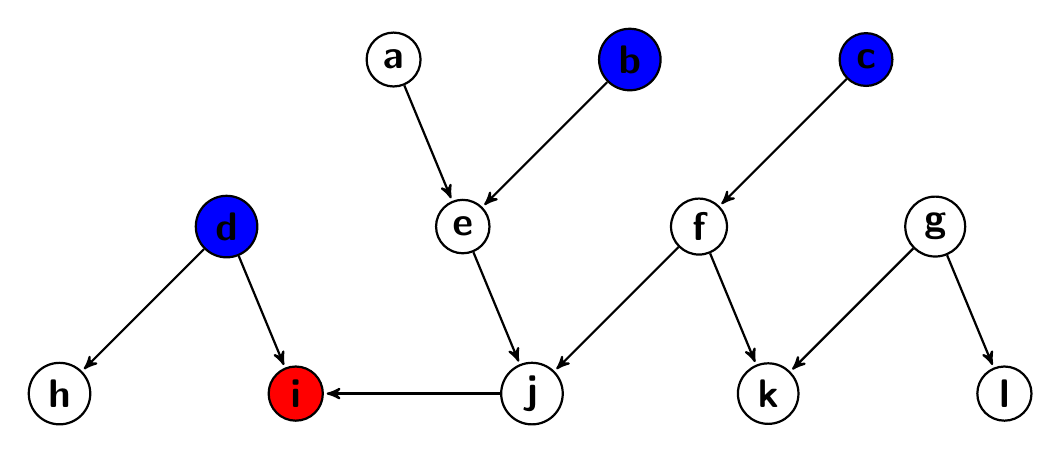
\begin{tikzpicture}[->,>=stealth',shorten >=1pt,auto,node distance=3cm,
                    thick,main node/.style={circle,draw,font=\sffamily\Large\bfseries}]
  \node[main node] (a) {a};
  \node[main node,fill=blue] (b) [right of=a] {b};
  \node[main node,fill=blue] (c) [right of=b] {c};
  \node[main node,fill=blue] (d) [below left of=a] {d};
  \node[main node] (e) [right of=d] {e};
  \node[main node] (f) [right of=e] {f};
  \node[main node] (g) [right of=f] {g};
  \node[main node] (h) [below left of=d] {h};
  \node[main node,fill=red] (i) [right of=h] {i};
  \node[main node] (j) [right of=i] {j};
  \node[main node] (k) [right of=j] {k};
  \node[main node] (l) [right of=k] {l};

  \path[every node/.style={font=\sffamily\small}]
    (a)
        edge node {} (e)
    (b)
        edge node {} (e)
    (c)
        edge node {} (f)
    (d)
        edge node {} (h)
        edge node {} (i)
    (e)
        edge node {} (j)
    (f)
        edge node {} (j)
        edge node {} (k)
    (g)
        edge node {} (k)
        edge node {} (l)
    (j)
        edge node {} (i)
    ;
\end{tikzpicture}
\caption{Example dependency graph}
\label{fig:dependency-graph}
\end{figure}

Similar to the dependency graph used in \ref{sub:codebook-based-event-correlation}, \cite{Gruschke_1998} suggests that a dependency graph can contain enough information to be used for event correlation, while also being simple to automatically generate. The dependency graph is a directed graph that maps the relationship managed objects. These objects can be hosts in a network, dependencies in a micro-service architecture, and so forth.
In figure \ref{fig:dependency-graph} we have mapped a series of objects as an example. Events are mapped to their corresponding object in the graph (colored in blue, object b, c and d). Then we walk the graph from those objects. As explained in \cite{Gruschke_1998}, when we optimally find one object node that are common for all the given events, we have most likely found the responsible node. In the example this is marked as red, object i.
\cite{Gruschke_1998} further outlines that the quality of the root-cause detection can be measured by the depth and length we need to walk the graph at. Objects that are further away from the initial object are less likely to be the root cause, and vica versa.
One of the main drawbacks of dependency graph based correlation is the fact that it does not handle multiple, non-related problems very well. \cite{Gruschke_1998} assumes that only one problem occurs at a time. If multiple problems occur that are not related or affect each other, finding the root-case may prove to be impossible, or select the wrong root-cause object.
Assumes the events are for a single fault. Meaning it will not be able to handle detecting multiple failing nodes.
As with the codebook-based event correlation we discussed in \ref{sub:codebook-based-event-correlation}, dependency graphs also lack the notion of time. Additionally the dependency graph is not taking advantage of attributes on the nodes to further enhance the graph.

\subsection{Bayesian Network Based Event Correlation}

Bayesian networks are one of the most widely used graphical models for representing and reasoning about the probabilistic causal relationships between variables\cite{Kavousi_2014}. Bayesian networks are usually represented by directed acyclic graphs. Directed acyclic graphs are finite directed graphs that contain no direct cycles. This means that there is no way to start from a given node, and via the directed edges return back to the same node. Each node in the network represents a variable of interest and the edges describe the relations between these variables.
The Bayesian network is split up into two parts. First there is the graphical model of the network which shows the nodes and the edges that connect them. Secondly, there is the conditional probability tables associated with each node. The table consist of the probabilities that a node is in a given state given the state of its parent nodes.



Both \cite{Kavousi_2014} and \cite{Qin_2004} utilize Bayesian networks to create "Bayesian attack graphs" (BAG) which are models that use Bayesian networks to depict the security attack scenarios in a system.

As a simple experiment using a Bayesian Network for detection, we have the directed acyclic graph as shown in Figure \ref{fig:simple-directed-acyclic-graph}. The nodes are a bit like the ones represented in Codebook-based correlation \ref{sub:codebook-based-event-correlation} where the nodes $B$ and $C$ represent two symptom events that are analyzed by the system, these can be events from an IDS, host machine logs, web logs, et cetera. The node $A$ represent a problem node and is not connected to any specific events. The purpose of this Bayesian network, is to answer the following question: What is the probability that, when we observe the two events $B$ and $C$, we have a problem $A$?

To calculate this, we first need the the conditional probability tables, which are given in Table \ref{tab:probabability-tables}.

\begin{figure}[ht]
\centering
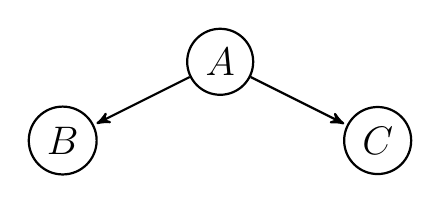
\begin{tikzpicture}[->,>=stealth',shorten >=1pt,auto,node distance=1cm,
                    thick,main node/.style={circle,draw,font=\sffamily\Large\bfseries}]
  \node[main node] (a) {$A$};
  \node[main node] (b) [below of=a,xshift=-2cm] {$B$};
  \node[main node] (c) [below of=a,xshift=2cm] {$C$};

  \path[every node/.style={font=\sffamily\small}]
    (a)
        edge node {} (b)
        edge node {} (c)
    ;
\end{tikzpicture}
\caption{Simple example directed acyclic graph}
\label{fig:simple-directed-acyclic-graph}
\end{figure}

\begin{table}[ht]
\centering
\begin{tabular}{|l|l|}
\hline
$P(A = 0)$ & $P(A = 1)$ \\ \hline
$0.8$ & $0.2$ \\ \hline
\end{tabular}
\begin{tabular}{|l|l|l|}
\hline
$A$ & $P(B = 1|A)$ & $P(B = 0|A)$ \\ \hline
$1$ & $0.9$ & $0.1$ \\ \hline
$0$ & $0.05$ & $0.95$ \\ \hline
\end{tabular}
\centering
\begin{tabular}{|l|l|l|}
\hline
$A$ & $P(C = 1|A)$ & $P(C = 0|A)$ \\ \hline
$1$ & $0.95$ & $0.05$ \\ \hline
$0$ & $0.05$ & $0.95$ \\ \hline
\end{tabular}
\caption{Conditional probability tables}
\label{tab:probabability-tables}
\end{table}

We can then calculate the probability that $A$ has occurred, given that we have observed the events $B$ and $C$ by using Bayes' theorem.
\begin{align*}
    &P(A=1 | B=1, C=1)\\
    &=\frac{P(A=1)P(B=1,C=1|A=1)}{P(B=1,C=1)}\\
    &=\frac{P(A=1)P(B=1,A=1)P(C=1,A=1)}{P(A=1)P(B=1|A=1)P(C=1|A=1)+P(A=0)P(B=1|A=0)P(C=1|A=0)}\\
    &=\frac{0.2\cdot0.9\cdot0.95}{(0.2\cdot0.9\cdot0.95)+(0.8\cdot0.05\cdot0.05)}\\
    &\approx 0.9884
\end{align*}
In this case, we see that there is a 98.8\% chance that the problem/alert $A$ has happened, by observing the arrival of the two events $B$ and $C$.


\subsection{Neural Network Approaches}
\subsection{Etc}



\section{Rule-based event correlation}
\label{sec:eventcorrelation}
\todo{Give an intro into the world of correlating events, why is it so valuable?}

\begin{itemize}
    \item Reduce alert-fatigue by generating high-fidelity alerts.
    \item Gather up smaller events that in and of them self are not worthy an alarm.
\end{itemize}

Rule-based event correlation software is historically known as a expert system. \cite{cronk_1988} defines an expert system as a "problem-solving software that embodies specialized knowledge in a narrow task domain to do work usually performed by a trained, skilled human.".

According to \cite{cronk_1988}, expert systems are organized around three levels; data, control and task knowledge. \todo{See figure 2 in paper. It should be incorporated in some way, as it pretty much defines how we have built MEC}.

Traditionally, creating the rules that goes into a knowledge base is in \cite{cronk_1988} defined as two-fold; first you have the subject-matter expert which has the expertise and knowledge about which events you are interested in creating correlations against, and secondly the knowledge engineer which is familiar with how the expert system works and how the rules has to be written to be understood by the system.
In more modern settings, usually the subject-matter expert is also able to write rules

What are some of the drawbacks of rule-based event correlation?

\begin{itemize}
    \item Doesn't learn or adapt
    \item Requires the subject-matter expert to define the rules, and the knowledge engineer to implement them
    \item Time-consuming to write and "push" rules into the system
    \item Requires testing and monitoring to make sure that:
    \begin{enumerate}
        \item the rule triggers on the intended events and
        \item the rule does not create tons of alerts that will flood the analysts handling the alerts
    \end{enumerate} 
    \item Maintenance of the rule repository is time-consuming
    \item Networks may differ, so it's not given that a rule that fits into one network, can automatically be used in another.
\end{itemize}

Regardless of all the drawbacks, we see a common trend that rule-based systems are the most common when it comes to network-based monitoring (see Suricata, Snort) as well as for log data in SIEMs like Splunk, ELK, OSSEC and OSSIM.


There exists several different types of software that makes it possible to correlate events in real-time based on log data.

Software based on event correlation commonly referenced in academia today is largely defunct or the source code is unavailable. 

\begin{itemize}
    \item Swatch and 2swatch - defunct, single-threaded. Last updated in 1997?
    \item logsurfer \cite{thompson_2017} written in C. Improves upon Swatch.
    \item Simple Event Correlator (SEC) is still being actively developed to this date. This is the software that is the most prominent in the literature that I have found. I will address that tool in its own separate section under \ref{sec:SEC}.
    \item Variable Temporal Event Correlator (VTEC) - Built custom for log monitoring and correlation at the company Advanced Micro Devices (AMD). Can not find source code. Feature distributed "workers" and a "variable server" that holds state. Written in Perl and the software uses Perl-based rules.
    \item Event Query Language (EQL). Part of Endgame/Elastic. Written in Python. Scales vertically, same as SEC. Implements a Abstract Syntax Tree for Windows Event Logs specifically.
    \item KSQL - Supports correlation based on time in a Kafka queue. Limited to Kafka as queuing technology.
    \item Splunk - One of the most popular Enterprise SIEM solutions. Supports writing "alerts" that allow time-based correlations.
\end{itemize}
There are several other correlation-based systems other than the ones mentioned above, but they employ some form of machine learning or statistical analysis instead of a rule-based approach. This is usually used for anomaly detection or "finding the unknown" in a dataset, which is not the focus of this thesis.

\subsection{Simple Event Correlator}
\label{sec:SEC}

In the research that I have found, SEC is the most commonly referenced and used software for event correlation across different syslog events. It is widely used, and has been deployed in several different sectors and industries (Finance, Telecom, IT security, Government, Retail, etc. \cite{vaarandi2005tools}) and utilized for several different purposes like fraud detection, insider-threat detection, system fault and availability and security events. SEC is quite versatile, as it is agnostic to the type of log event that it receives. SEC uses rules that are using Perl-style regular expressions for matching events and extracting data from the event itself using sub-expressions. The extracted data can then be used to correlate between other matching events.

However, even though SEC is popular and commonly used, there are several improvements that could be done. Some of the constraints include:
\begin{itemize}
    \item Heavily based on regular expressions for writing rules, which makes it both hard to analyze rules, modifying existing rules and writing new rules.
    \item Current version can only be scaled vertically. The context-state used for correlation is per-process only and therefore any and all correlation between events have to happen in the same process. It is possible to use SEC in a multi-process fashion to handle separate log types, but this removes the possibility to correlate between those log types. 
    \item Few open source rules and rule-sets. The analyst generally has to start from scratch writing their own rules
    \item Limited support for multi-line logs
    \item Windows Event Logs has to be converted to syslog
    \item Made generic, not specific for Windows Event Logs
\end{itemize}

\subsection{Event Query Language}
\label{sec:eql}

Part of Endgame/Elastic. Written in Python. Scales vertically, same as SEC. Implements a Abstract Syntax Tree for Windows Event Logs specifically.

Is parsed "after the fact".


\section{Windows Event Log}

Windows Event Log is a built-in capability in the Microsoft Windows operating systems. The different event log categories can be configured using Group Policy Objects in an enterprise. The total amount of logs generated on a system is huge, so configuration is necessary to remove noisy or uninteresting events.
There are events for "everything". \todo{Find some examples here}
Windows Event Logs are usually sent to a centralized location for storage and analysis, either using the built-in option called Windows Event Log Forwarding or using custom agents like Splunk Universal Forwarder, winlogbeat or nxlog to name a few.

\subsection{Sysmon}
Sysmon is an extension to the stock Windows Event Log and allows for a more powerful customization of what events go into the event log. Using a kernel driver, Sysmon is able to add support for a wider variety of interesting events. The table \ref{tab:sysmoneventtypes} is a list of each event type that Sysmon can generate.

\begin{table}[ht]
\begin{tabular}{l|l}
ID & Description \\ \hline
1 & Process creation \\
2 & A process changed a file creation time \\
3 & Network connection \\
4 & Sysmon service state changed \\
5 & Process terminated \\
6 & Driver loaded \\
7 & Image loaded \\
8 & CreateRemoteThread \\
9 & RawAccessRead \\
10 & ProcessAccess \\
11 & FileCreate \\
12 & RegistryEvent (Object create and delete) \\
13 & RegistryEvent (Value Set) \\
14 & RegistryEvent (Key and Value Rename) \\
15 & FileCreateStreamHash \\
17 & PipeEvent (Pipe Created) \\
18 & PipeEvent (Pipe Connected) \\
19 & WmiEvent (WmiEventFilter activity detected) \\
20 & WmiEvent (WmiEventConsumer activity detected) \\
21 & WmiEvent (WmiEventConsumerToFilter activity detected) \\
22 & DNSEvent (DNS query) \\
255 & Error
\end{tabular}
\caption{List of Sysmon event types}
\label{tab:sysmoneventtypes}
\end{table}

\section{MITRE Cyber Analytics Repository}
"The MITRE Cyber Analytics Repository (CAR) is a knowledge base of analytics developed by MITRE based on the MITRE ATT\&CK adversary model"

One of the CAR analytics is "CAR-2013-04-002: Quick execution of a series of suspicious commands". This analytic is based on the assumption that certain commands are frequently ran by malicious actors on a system, while regular users do not run them. CAR-2013-04-002 outlines several commands of interest:
\begin{multicols}{2}
\begin{itemize}
\item arp.exe
\item at.exe
\item attrib.exe
\item cscript.exe
\item dsquery.exe
\item hostname.exe
\item ipconfig.exe
\item mimikatz.exe
\item nbstat.exe
\item net.exe
\item netsh.exe
\item nslookup.exe
\item ping.exe
\item quser.exe
\item qwinsta.exe
\item reg.exe
\item runas.exe
\item sc.exe
\item schtasks.exe
\item ssh.exe
\item systeminfo.exe
\item taskkill.exe
\item telnet.exe
\item tracert.exe
\item wscript.exe
\item xcopy.exe
\end{itemize}
\end{multicols}
\url{https://car.mitre.org/analytics/CAR-2013-04-002/}



\section{Sigma}
\url{https://github.com/Neo23x0/sigma}

Sigma is an open standard for rules that are used to generically describe searches in log data. It is primarily used as a high-level rule that transcompile into SIEM queries like Splunk, ElasticSearch, QRadar, etc. The rules are written in YAML (Yet Another Markup Language), and are key-value based.
\\
The following example Sigma rule is a basic rule that detects running \lstinline{ipconfig}, \lstinline{arp} and \lstinline{echo} within a ten second timeframe, filtered by the \lstinline{MachineName} key in the event: \todo{We should add some examples of what an event actually looks like, to make it more obvious to the reader what we are talking about here}

\begin{lstlisting}[
    basicstyle=\small
]
title: Quick Execution of a Series of Suspicious Commands
id: 61ab5496-748e-4818-a92f-de78e20fe7aa
description: Detects multiple suspicious process in a limited timeframe
status: experimental
references:
    - https://car.mitre.org/wiki/CAR-2013-04-002
author: Martin Ingesen
modified: 2020/01/01
tags:
    - car.2013-04-002
logsource:
    category: process_creation
    product: windows
detection:
    selection:
        CommandLine:
            - ipconfig
            - arp
            - echo
    timeframe: 10s
    condition: selection | count() by MachineName > 3
falsepositives:
    - False positives depend on scripts and
    administrative tools used in the monitored environment
level: low
\end{lstlisting}
The format contains some required and some optional fields, and is extensible with our own custom fields.

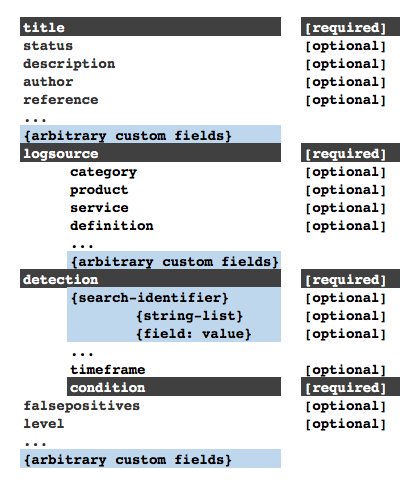
\includegraphics[scale=0.525]{figures/new-rule-format/Sigma_Schema.png}

Image source: \url{https://github.com/Neo23x0/sigma/wiki/Specification}
\chapter{Methodology}
\label{chap:methodology}

\iffalse
The type of research you did
How you collected your data
How you analyzed your data
Any tools or materials you used in the research
Your rationale for choosing these methods
\fi

\anders{Vil bare understreke at du kanskje er ute etter en vitenskapelig metode her, ikke å gå inn på hvorfor du valgte Go. Go er implmentasjonen din, mer på begrunnelse i en beskrivelse av valg av verktøy for performance reasons or whatnot. Når jeg leser methodology i en vitenskapelig oppgave/artikkel/avhandling så skal det gå på om du f.eks. utvikler noe nytt, bidrar til en felles forståelse om bedring av et eksisterende miljø eller noe sånt svada.}

\section{The Go programming language}

\com{Her er en rask intro, argumentasjonen hvorfor vi valgte dette finner du i eksperiment XYZ}
\todo{Why did we choose Go?} \com{Dette er ikke teori/bakgrunn, men mer et metodevalg.}
\subsection{Goroutines}
\todo{What are these lightweight Go threads?}\\
Goroutines are lightweight threads that are handled by the Go runtime.
\subsection{Channels}

\todo{What are channels? What are some of the considerations we have to take when working with them?}\\
\todo{Are there any best practices?}\\
Channels are the preferred way to communicate between Goroutines in Go.

\subsection{Concurrency vs parallelism}
\todo{Discuss why Go is concurrent, but not parallel}
\chapter{Experiment}
\label{chap:experiment}
The following chapter introduce our improved implementation based on the methodology presented in Chapter \ref{chap:methodology}. The dataset collection and required preprocessing is presented, the software and hardware specifications.......

\iffalse
The following chapter introduces the actual implementation of the experiment based on the methodology presented in Chapter 4. The collection of the data set, the software versions, the hardware
specifications and the used algorithms during the experiment are presented as well as the experimental design and the technical implementation. It demonstrates the technical execution of the
methodology for reproducibility of the use case.
\fi

\section{Software Specifications}
\label{sec:softwarespecs}

\begin{itemize}
    \item Ubuntu 18.04.4 LTS Released February 2020
    \item go version go1.13.3 linux/amd64, released October 2019
    \item Perl v5.30.2 built for x86\_64-linux, march 2020
\end{itemize}

\section{Hardware Specifications}
\label{sec:hardwarespecs}
The host system used for running the experiments feature a Intel(R) Core(TM) i7-7600U CPU @ 2.80GHz processor and 24 GB memory. The processor features two physical cores, and is capable of running two threads per core. This means that the processor has a maximum of 4 logical cores.

\section{Dataset}

\section{Dataset preprocessing}
\label{sec:datasetprocessing}

The Mordor-dataset require us to do some pre-processing to ingest it into Simple Event Correlator. Since our own solution is supposed to mirror SEC, 

\section{Implementation that uses Simple Event Correlators own rule format (regex based)}
\todo{Why did we choose Go?}

\subsection{SEC rule format}
\n{Move this section somewhere else}
\begin{lstlisting}
type=single
ptype=regexp
pattern=(\S+)sshd.*
desc=This is a description
\end{lstlisting}

\subsubsection{type}
Type of rule. There are many different types here.
I have focused on rules using "SingleWithThreshold" which takes an action if there are X number of matches in Y time.

Single

Suppress

Calendar

SingleWithSuppress

Pair

PairWithWindow

SingleWith2Thresholds

EventGroup

SingleWithScript

Jump

\subsubsection{ptype}
Pattern type. RegExp is a Perl regular expression. Can use variables.

SubStr

PerlFunc

Cached

TValue

\subsubsection{pattern}
The pattern that the log line will we tested against. The value of this pattern is based on the ptype. For example, if the ptype is set to "RegExp", the pattern will be a Perl regular expression.

\subsubsection{desc}
Description field. But used for defining "scopes" when correlating.

\subsubsection{action}
The action to take when the rule "hits".

\subsubsection{continue}

\subsubsection{context}

\subsection{Implementation}
As discussed in chapter X, the programming language Go was chosen for implementing our new program to analyze our datasets. I have chosen to only implement the SingleWithTreshold type, and the RegExp pattern type (ptype). The "SingleWithTreshold" type triggers an action if there are X number of matches within Y time. We consider this to be the most usable rule type for our purpose. \com{What is the purpose?} For the pattern type, we choose to use "RegExp", which are Perl regular expressions. We consider this to be the best option for matching against syslog-based log lines.

Other than the fact that Go is a compiled language and Perl is a interpreted language, the main additions in our implementation is that our version:
\begin{itemize}
    \item Uses Go channels for re-injecting events into the context engine.
    \item The use of channels and goroutines gives us the ability to run in a threaded matter, utilizing multiple cores.
\end{itemize}

\subsubsection{Workers}
\todo{What are workers?}

\section{Implemented a new rule format}
This format relies less on the extensive use of Regexes \com{Hvorfor er dette en fordel? Hvorfor er dette valget smart? Beskriv dette i experiment delen?}, as we saw in the rules used by Simple Event Correlator. \todo{Elaborate on this}
\\
For each log line/event we:

\begin{enumerate}
    \item Tokenize the event into a Event struct. \com{Hva er dette?... Flytt beskrivelsen opp til Experiment i stedet?}
    \item Iterate over every rule, checking if the Event matches the detection-part of the rule.
    \begin{itemize}
        \item If there is a match, we run the Event through the context engine, to see if the conditions are met for the rule.
    \end{itemize}
\end{enumerate}

When we tokenize the event, we take a single line of log/event, and split it into its key-value representation. For instance, the following event log is a single line of text:
\begin{lstlisting}[breaklines=true]
<14>Feb 18 02:29:49 Client02.mrtn.lab Microsoft-Windows-Sysmon[2092]: Process Create:  RuleName:   UtcTime: 2020-02-18 10:29:49.839  ProcessGuid: {dadb16ad-bc9d-5e4b-0000-0010c8fd3600}  ProcessId: 1040  Image: C:\Windows\System32\whoami.exe  FileVersion: 10.0.17763.1 (WinBuild.160101.0800)  Description: whoami - displays logged on user information  Product: Microsoft Windows Operating System  Company: Microsoft Corporation  OriginalFileName: whoami.exe  CommandLine: whoami  CurrentDirectory: C:\Users\mrtn\  User: MRTNLAB\mrtn  LogonGuid: {dadb16ad-2c2d-5e17-0000-0020fc3c1b00}  LogonId: 0x1B3CFC  TerminalSessionId: 1  IntegrityLevel: Medium  Hashes: MD5=43C2D3293AD939241DF61B3630A9D3B6,SHA256=1D5491E3C468EE4B4EF6EDFF4BBC7D06EE83180F6F0B1576763EA2EFE049493A,IMPHASH=7FF0758B766F747CE57DFAC70743FB88  ParentProcessGuid: {dadb16ad-2cf1-5e17-0000-001027122b00}  ParentProcessId: 2748  ParentImage: C:\Users\mrtn\test.exe  ParentCommandLine: .\test.exe
\end{lstlisting}
But after tokenization, it looks like this:
\begin{lstlisting}[breaklines=true]
MachineName: Client02.mrtn.lab
ProcessType: Process Create: 
RuleName:   
UtcTime: 2020-02-18 10:29:49.839
ProcessGuid: {dadb16ad-bc9d-5e4b-0000-0010c8fd3600}
ProcessId: 1040
Image: C:\Windows\System32\whoami.exe
FileVersion: 10.0.17763.1 (WinBuild.160101.0800)
Description: whoami - displays logged on user information  Product: Microsoft Windows Operating System
Company: Microsoft Corporation 
OriginalFileName: whoami.exe
CommandLine: whoami
CurrentDirectory: C:\Users\mrtn\
User: MRTNLAB\mrtn
LogonGuid: {dadb16ad-2c2d-5e17-0000-0020fc3c1b00}
LogonId: 0x1B3CFC
TerminalSessionId: 1
IntegrityLevel: Medium
Hashes: MD5=43C2D3293AD939241DF61B3630A9D3B6,SHA256=1D5491E3C468EE4B4EF6EDFF4BBC7D06EE83180F6F0B1576763EA2EFE049493A,IMPHASH=7FF0758B766F747CE57DFAC70743FB88
ParentProcessGuid: {dadb16ad-2cf1-5e17-0000-001027122b00}
ParentProcessId: 2748
ParentImage: C:\Users\mrtn\test.exe
ParentCommandLine: .\test.exe
\end{lstlisting}
The tokenized version of the event log is stored as a Go struct, which makes it simpler to query specific parts of the event log directly, instead of having to parse the whole event log every time we want to access a single key-value pair. An example would be if we wanted to access the MachineName or CommandLine values from the above example, which would be done like this:  \lstinline{event['MachineName']} and \lstinline{event['CommandLine']}.


\subsection{Context}
\n{What is context?}
\\
When we want to do correlation between two or more events based on a rule, we need to have some kind of overview of what state our rule is in. When a new event arrives that triggers our rule, we need to know if this is the first event, if there are other events that have triggered before it, and most importantly, if the previous events that triggered the rule is within the given time frame of the rule. This is what we call "context".

\subsection{The Context Engine}
One of the benefits of our new implementation is the ability to process events concurrently. But when working with a context that is accessed by several workers concurrently, data races may appear. A data race occurs when two goroutines concurrently accesses the same variable (in this case the context variable), and at least one of the goroutines writes to the variable. The danger here is that we could have two or more goroutines with their own versions of the context that are out of sync. This could lead to data loss and/or a failure to detect when a rule-condition is met. The standard way of dealing with data races like this is to use a mutex. A mutex provides a locking mechanism to ensure that only one goroutine can manipulate a variable at a time.

In our implementation we have integrated a mutex in two different ways, using a shared context mutex and using a rule-based context mutex. \com{Det er ikke så interessant at vi har brukt to forskjellige, men hva oppnår vi? Hva var hensikten med dette?}

\subsubsection{Shared context}

For the shared context, we have a large map that looks like this:
\begin{lstlisting}
context := map[string]{
    Events  []Event
}
\end{lstlisting}
We access it by doing:
\begin{lstlisting}
c := context["CONTEXT_FOR_RULE_1"]
\end{lstlisting}
the variable \lstinline{c} now contain an array of \lstinline{event}s, if there are any for the given key \lstinline{CONTEXT_FOR_RULE_1}. In our implementation we use the ID of the rule for this lookup, as it is an (Universally unique identifier) UUID4-string, and is safe to use as a unique identifier.


Since we may both read and write to the \lstinline{c} variable, we need to lock a mutex for the \lstinline{context} map. We can do this like this:

\begin{lstlisting}
context := map[string]{
    Events  []Event
}
contextMutex := &sync.RWMutex{}

contextMutex.Lock()
c := context["CONTEXT_FOR_RULE_1"]

// Add or remove events to the context here

context["CONTEXT_FOR_RULE_1"] = c

contextMutex.Unlock()
\end{lstlisting}

We now have a goroutine-safe way of accessing and editing our context. The drawback of this is in the design, when multiple goroutines try to access the context, they will have to wait for their turn to lock on the context.

\subsubsection{Rule-based context}
For the rule-based context, both the context and the context mutex is defined in the rule struct itself:
\begin{lstlisting}
type context struct {
    events []event
}

type Rule struct {
	Context        context
	ContextMutex   sync.RWMutex
	Title          string
	ID             string
	...
}
\end{lstlisting}
Accessing and modifying the rule context is pretty similar to the shared context mutex, but instead of the shared context, we are accessing \lstinline{rule} instead:
\begin{lstlisting}
rule.ContextMutex.Lock()
c := rule.Context

// Add or remove events to the context here

rule.Context = c

rule.ContextMutex.Unlock()
\end{lstlisting}


The benefit to doing it this way is clear. If several goroutines are accessing the context at the same time, but are interested in different rules, we will lock on the individual rule mutex instead of a single shared mutex.

There may still be cases when multiple goroutines try to lock on the same rule and have to wait in line. So depending on the number of rules and how often the rules are triggered we may see performance equal to the shared context as a worst case scenario.
\chapter{Results {\&} Analysis}
\label{chap:resultsanalysis}
In this chapter the results of both experiments, introduced in Chapter \ref{chap:experiment}, are presented and analysed.

\section{Implementation that uses Simple Event Correlators own rule format (regex based)}

\begin{figure}[ht]
\centering
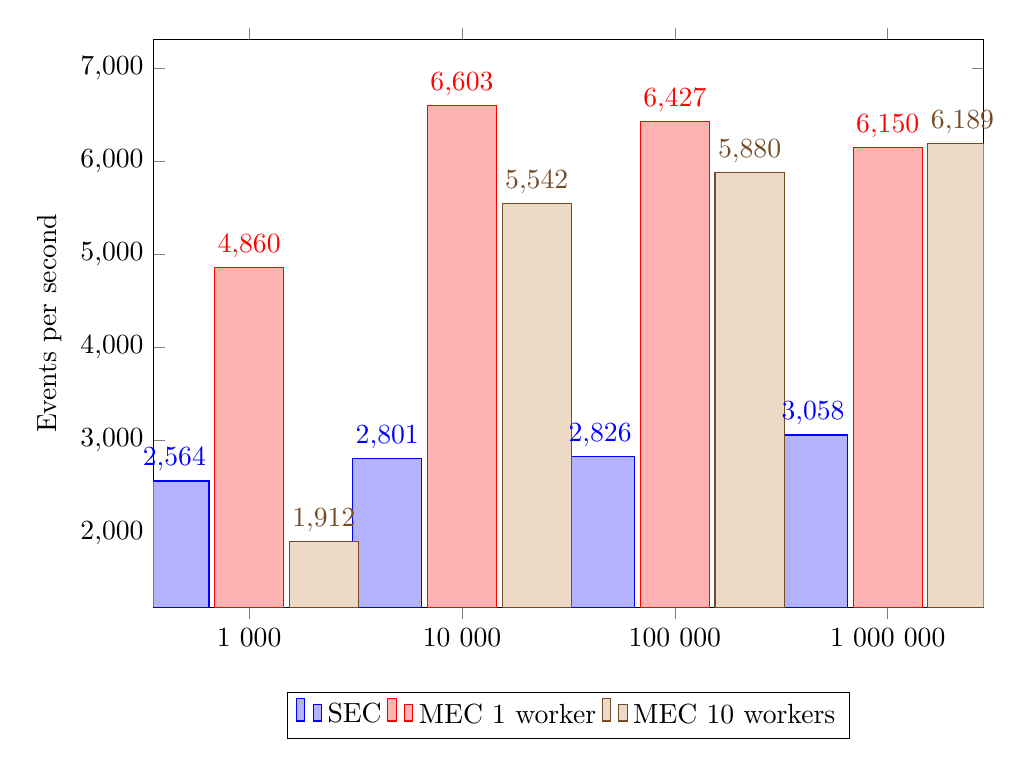
\begin{tikzpicture}
\begin{axis}[
    xtick=data,
	height=250pt,
	ylabel=Events per second,
	enlargelimits=0.15,
	legend style={at={(0.5,-0.15)},
	anchor=north,legend columns=-1},
	ybar,
	bar width=25pt,
	symbolic x coords={1 000, 10 000, 100 000, 1 000 000},
	nodes near coords,
	nodes near coords style={above}
]
\addplot coordinates {(1 000,2564) (10 000,2801) (100 000,2826) (1 000 000,3058)}; % SEC
\addplot coordinates {(1 000,4860) (10 000,6603) (100 000,6427) (1 000 000,6150)}; % MEC1W
\addplot coordinates {(1 000,1912) (10 000,5542) (100 000,5880) (1 000 000,6189)}; % MEC10W
\legend{SEC, MEC 1 worker, MEC 10 workers}
\end{axis}
\end{tikzpicture}
\caption{Baseline dataset}
\label{fig:baseline-perf}
\end{figure}


\begin{figure}[ht]
\centering
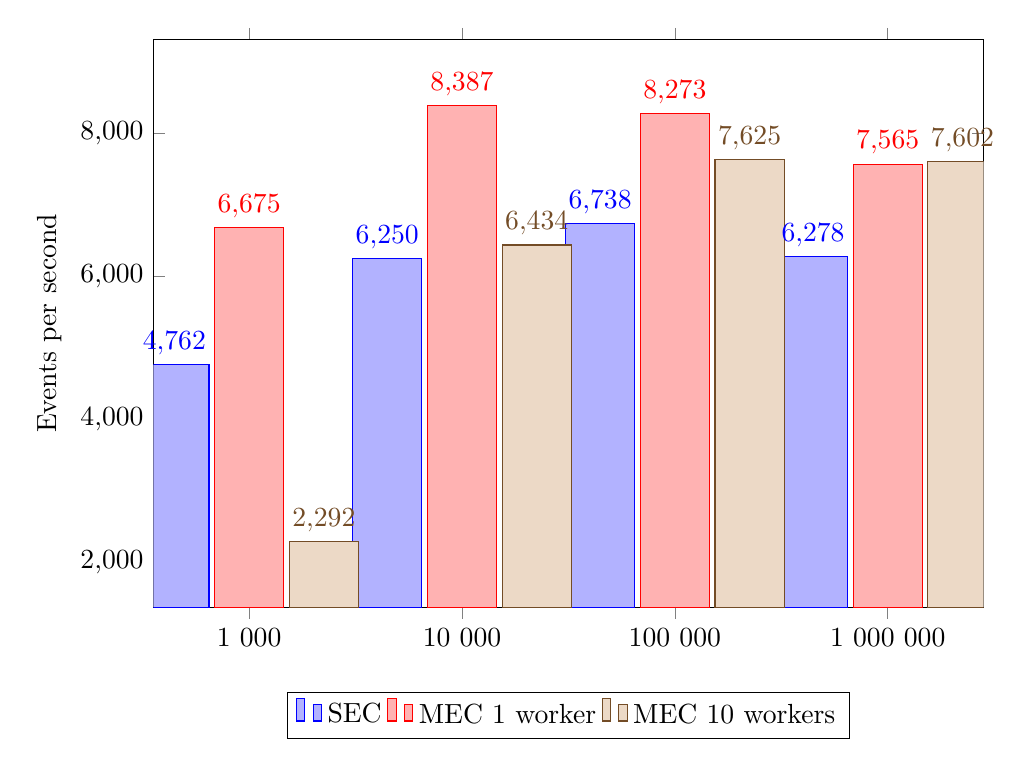
\begin{tikzpicture}
\begin{axis}[
    xtick=data,
	height=250pt,
	ylabel=Events per second,
	enlargelimits=0.15,
	legend style={at={(0.5,-0.15)},
	anchor=north,legend columns=-1},
	ybar,
	bar width=25pt,
	symbolic x coords={1 000, 10 000, 100 000, 1 000 000},
	nodes near coords,
	nodes near coords style={above}
]
\addplot coordinates {(1 000,4762) (10 000,6250) (100 000,6738) (1 000 000,6278)}; % SEC
\addplot coordinates {(1 000,6675) (10 000,8387) (100 000,8273) (1 000 000,7565)}; % MEC1W
\addplot coordinates {(1 000,2292) (10 000,6434) (100 000,7625) (1 000 000,7602)}; % MEC10W
\legend{SEC, MEC 1 worker, MEC 10 workers}
\end{axis}
\end{tikzpicture}
\caption{High signal low noise dataset}
\label{fig:high-signal-low-noise}
\end{figure}


\begin{figure}[ht]
\centering
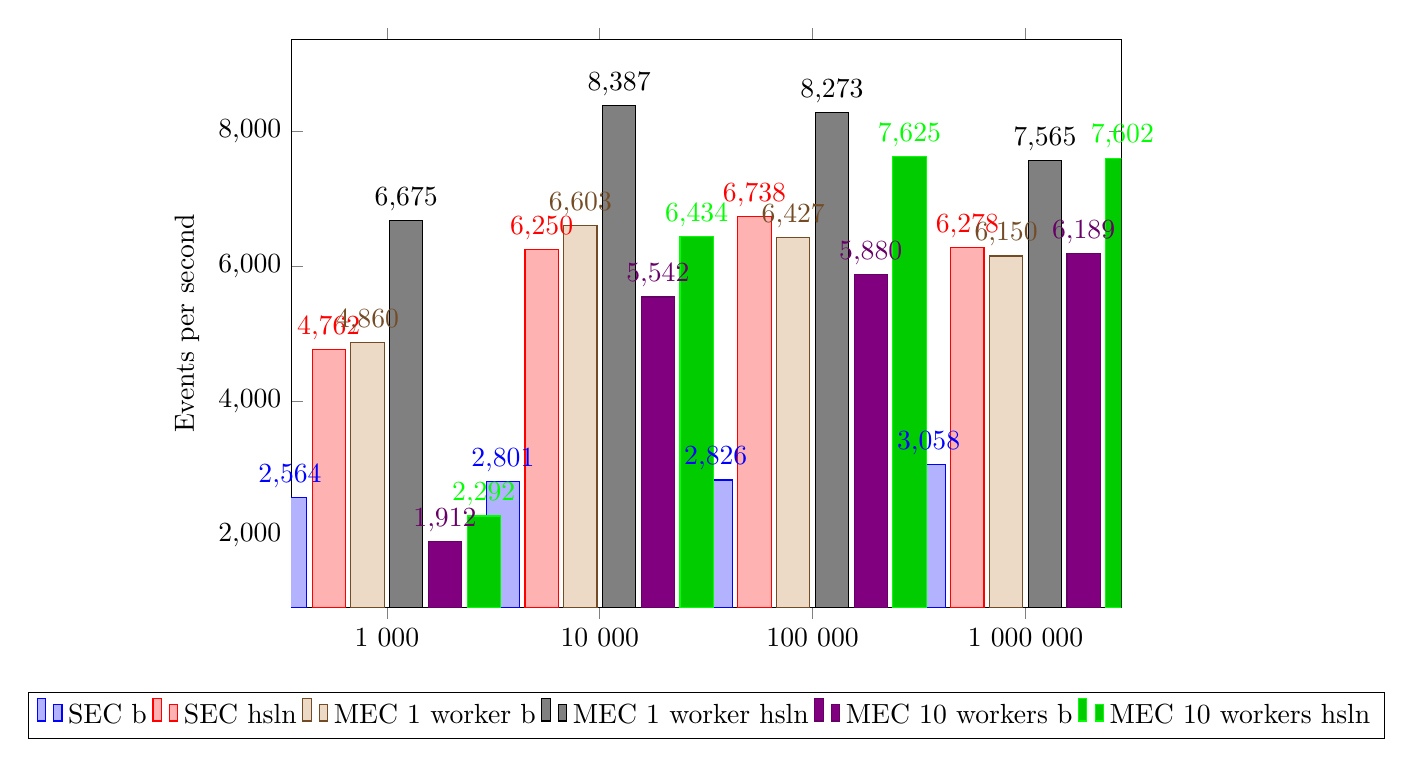
\begin{tikzpicture}
\begin{axis}[
    xtick=data,
	height=250pt,
	ylabel=Events per second,
	enlargelimits=0.15,
	legend style={at={(0.5,-0.15)},
	anchor=north,legend columns=-1},
	ybar,
	bar width=12pt,
	symbolic x coords={1 000, 10 000, 100 000, 1 000 000},
	nodes near coords,
	nodes near coords style={above}
]
\addplot coordinates {(1 000,2564) (10 000,2801) (100 000,2826) (1 000 000,3058)}; % SEC baseline
\addplot coordinates {(1 000,4762) (10 000,6250) (100 000,6738) (1 000 000,6278)}; % SEC high signal low noise

\addplot coordinates {(1 000,4860) (10 000,6603) (100 000,6427) (1 000 000,6150)}; % MEC1W baseline
\addplot coordinates {(1 000,6675) (10 000,8387) (100 000,8273) (1 000 000,7565)}; % MEC1W high signal low noise

\addplot coordinates {(1 000,1912) (10 000,5542) (100 000,5880) (1 000 000,6189)}; % MEC10W baseline
\addplot coordinates {(1 000,2292) (10 000,6434) (100 000,7625) (1 000 000,7602)}; % MEC10W high signal low noise

\legend{SEC b, SEC hsln, MEC 1 worker b, MEC 1 worker hsln, MEC 10 workers b, MEC 10 workers hsln}
\end{axis}
\end{tikzpicture}
\caption{Comparing baseline (b) and High signal low noise (hsln) dataset}
\label{fig:comparing-perf}
\end{figure}

\subsection{Results}
We want to see if our Go implementation can out-perform SEC when handling a high signal, low noise dataset. The Figures \ref{fig:high-signal-low-noise}, \ref{fig:baseline-perf} and \ref{fig:comparing-perf} shows the results for that:
\\

\\
These tests are run with 1 logical core on a "Intel(R) Core(TM) i7-7600U CPU @ 2.80GHz" (2 cores x 2 threads per core = max 4 logical cores) and 24GB RAM.\\
\textbf{What can we say about the performance difference between the two datasets?}\\
It's because of the implementation in SEC and MEC, if we match a rule quickly, we don't have to check all the other rules for a match, and this saves time.\\
\textbf{Why is the MEC10W slower in the start?}\\
Since MEC10W launches ten workers using Go routines, the additional overhead involved with that process is slowing down the performance if you compare it with "single-worker"-style implementations like SEC or MEC with 1 worker.\\
\textbf{Why are the runs on the 1 000 dataset generally lower?}
Because of the small dataset used (1 000), the time spent on general initialization is spread across a lot fewer events, which decreases the events/second throughput.

\subsubsection{Multiple cores}

By using all CPU cores available (4) instead of a single one, we can take better advantage of Gos concurrency model, and raise the throughput when using multiple workers and CPUs as seen in Figure \ref{fig:multicore-hsln-perf} and \ref{fig:multicore-b-perf}.\\
\textbf{What can we say about 1CPU,10W "catching up" to the others around 100 000 events?}\\
This is pretty much the same as what we saw in the single core test.\n{ref her}. The time used to spin up the 10 workers (Go routines) is only outweighed at approximately 100 000 events. This is also why we are seeing a dip when using a dataset of 1 000 events.\\
\textbf{Why are the results of 1CPU,1W, 1CPU,10W and 10CPU,1W generally the same?}\\
This is because they in general are the same. When we are limiting our script to 1 worker, it doesn't really matter how many cores we use, as only one core will be running the worker regardless. There is however a slight benefit to the 4CPU,10W which we can clearly see from the Figure at 1 000 events. The main-function in Go is itself a Go routine, so when we are creating a worker in another core, the main-function can work uninterrupted with reading the log files, while the worker is not blocking since it is running in another core.

\begin{figure}[ht]
\centering
\pgfplotsset{scaled y ticks=false}
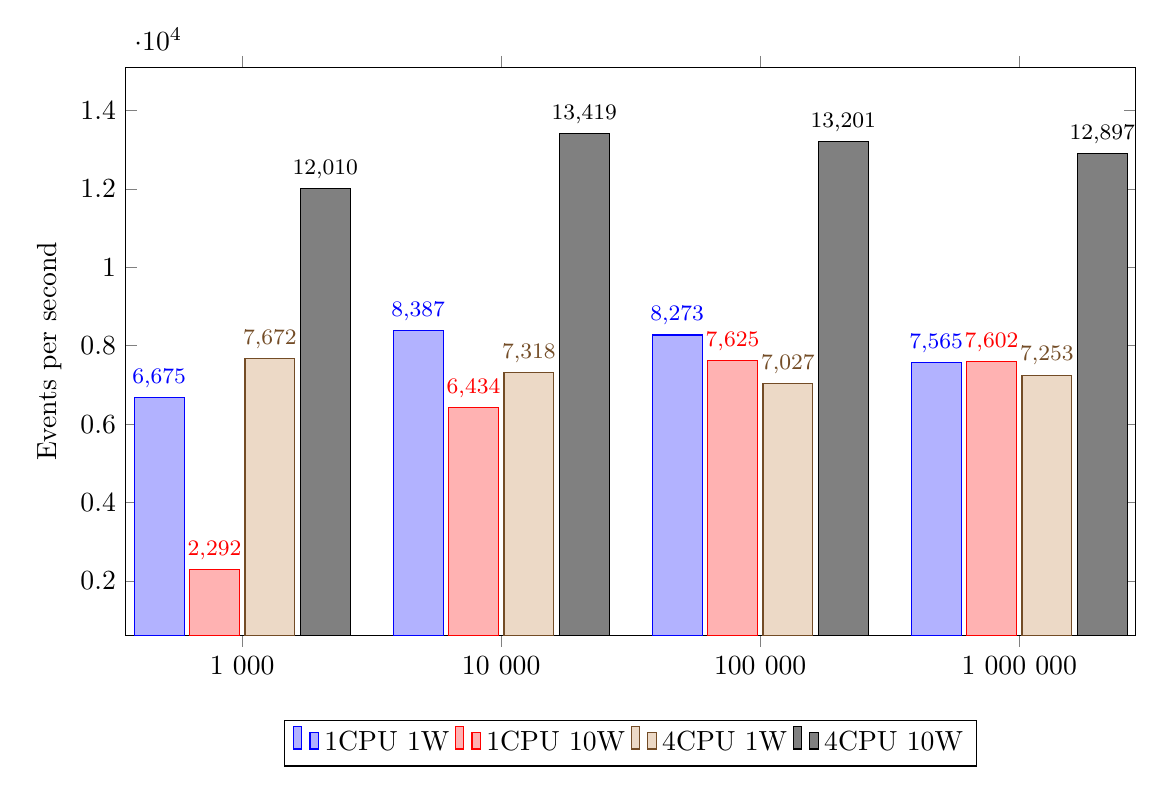
\begin{tikzpicture}
\begin{axis}[
    xtick=data,
    width=410pt,
	height=250pt,
	ylabel=Events per second,
	enlargelimits=0.15,
	legend style={at={(0.5,-0.15)},
	anchor=north,legend columns=-1},
	ybar,
	bar width=18pt,
	symbolic x coords={1 000, 10 000, 100 000, 1 000 000},
	nodes near coords,
	nodes near coords style={above, font=\footnotesize},
]
\addplot coordinates {(1 000,6675) (10 000,8387) (100 000,8273) (1 000 000,7565)}; % 1CPU 1W
\addplot coordinates {(1 000,2292) (10 000,6434) (100 000,7625) (1 000 000,7602)}; % 1CPU 10W
\addplot coordinates {(1 000,7672) (10 000,7318) (100 000,7027) (1 000 000,7253)}; % 4CPU 1W
\addplot coordinates {(1 000,12010) (10 000,13419) (100 000,13201) (1 000 000,12897)}; % 4CPU 10W
\legend{1CPU 1W , 1CPU 10W , 4CPU 1W , 4CPU 10W}
\end{axis}
\end{tikzpicture}
\caption{Concurrency with high signal low noise dataset}
\label{fig:multicore-hsln-perf}
\end{figure}

\begin{figure}[ht]
\centering
\pgfplotsset{scaled y ticks=false}
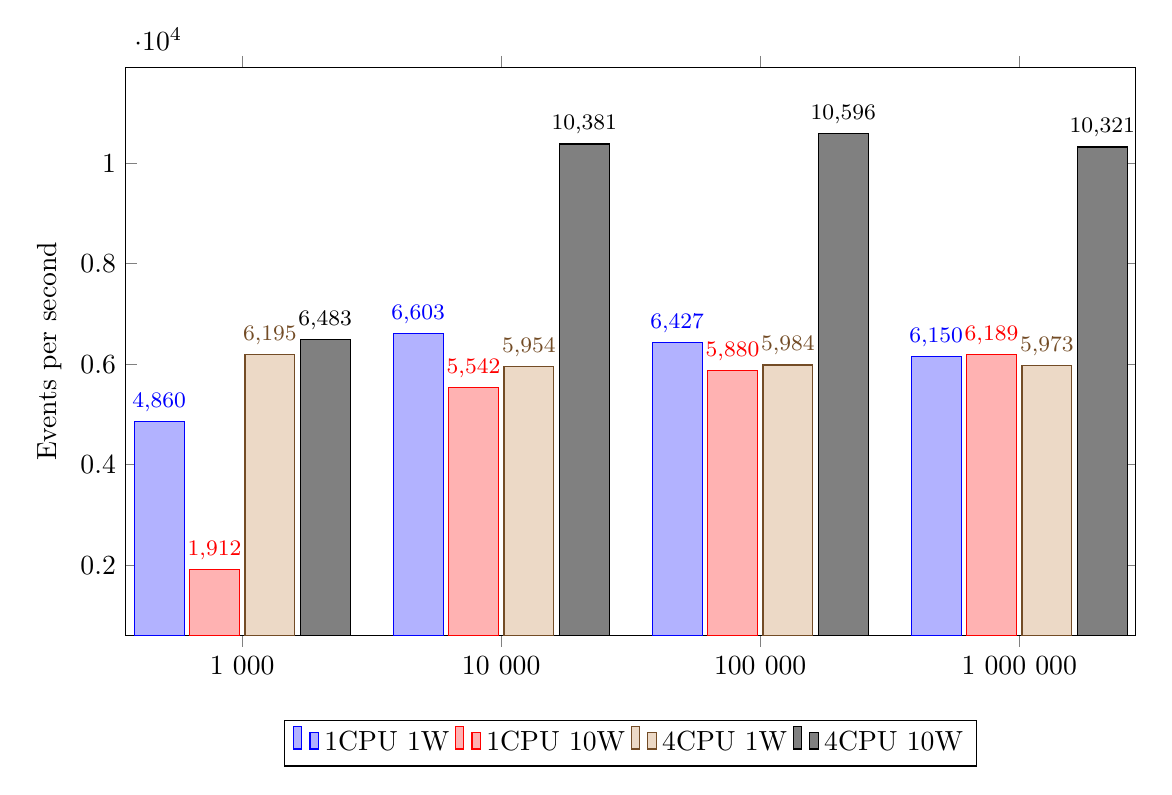
\begin{tikzpicture}
\begin{axis}[
    xtick=data,
    width=410pt,
	height=250pt,
	ylabel=Events per second,
	enlargelimits=0.15,
	legend style={at={(0.5,-0.15)},
	anchor=north,legend columns=-1},
	ybar,
	bar width=18pt,
	symbolic x coords={1 000, 10 000, 100 000, 1 000 000},
	nodes near coords,
	nodes near coords style={above, font=\footnotesize},
]
\addplot coordinates {(1 000,4860) (10 000,6603) (100 000,6427) (1 000 000,6150)}; % 1CPU 1W
\addplot coordinates {(1 000,1912) (10 000,5542) (100 000,5880) (1 000 000,6189)}; % 1CPU 10W
\addplot coordinates {(1 000,6195) (10 000,5954) (100 000,5984) (1 000 000,5973)}; % 4CPU 1W
\addplot coordinates {(1 000,6483) (10 000,10381) (100 000,10596) (1 000 000,10321)}; % 4CPU 10W
\legend{1CPU 1W , 1CPU 10W , 4CPU 1W , 4CPU 10W}
\end{axis}
\end{tikzpicture}
\caption{Concurrency with baseline dataset}
\label{fig:multicore-b-perf}
\end{figure}

\section{Implemented a new rule format}


\subsection{Results}
We are interested in seeing if there are any performance benefits from running our new rule implementation versus the re-implementation of the SEC rules. In the following graph we are running with only a single rule, using our high signal, low noise dataset. The bars labeled "SEC" are our re-implementation of the regular expression-based rules. "Original SEC" is Simple Event Correlator. "MEC" is our implementation with the new rule format.

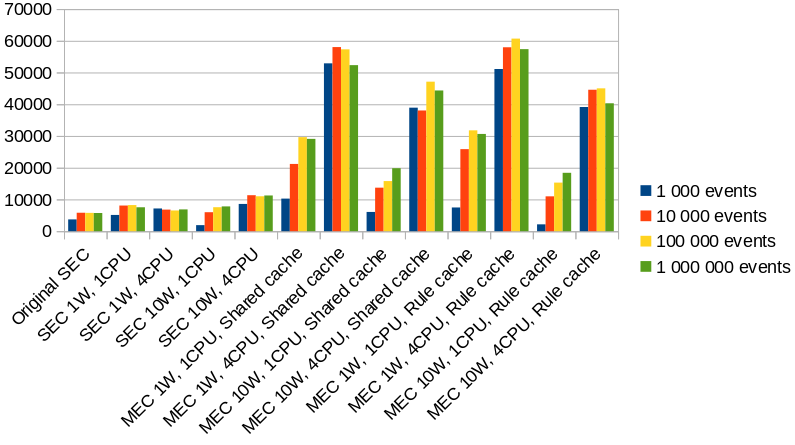
\includegraphics[scale=0.525]{figures/new-rule-format/performance.png}
\\
First of all, we see that our new rule format has in general increased the event throughput substantially. One interesting thing is that there is little to no difference between shared context locking and the rule-based locking in our implementation.

\todo{What happened with 1 000 events for MEC 10W,1CPU rule context locking here?..}

The reason for this could be that we are only using a single rule, so we are not actually benefiting from the different context locking logic that we have implemented. To further explore this, we have generated 1 000 rules randomly, and re-ran our high signal, low noise dataset against them.

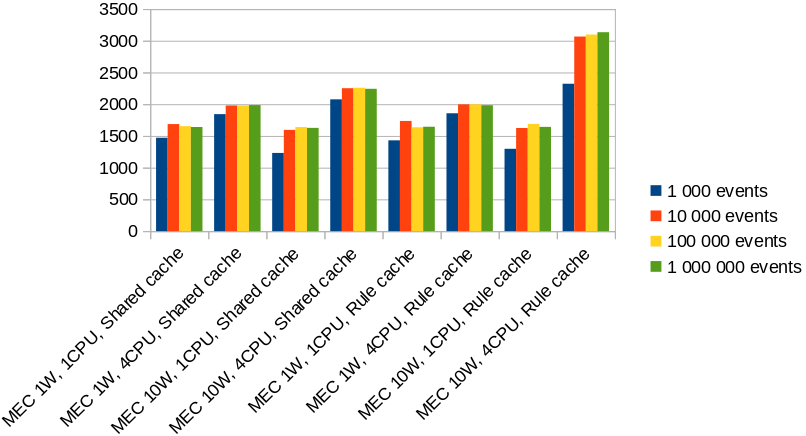
\includegraphics[scale=0.525]{figures/new-rule-format/performance-2.png}
\\
In the above graph, we see a drastic fall in events processed per second, because of the need to iterate over more rules. As expected, we see that rule-cache with 10W and 4CPU gives a 39.77\% increase compared against 10W, 4CPU and shared locking.

What is interesting here is the little difference between (1W, 1CPU), (10W, 1CPU), (1W, 4CPU) and the two different locking implementations. This makes sense, as the low amount of workers don't take advantage of the rule-based context locking, and will then fall to the same speed as shared context locking.

\subsubsection{Low signal, high noise dataset}
\todo{This experiment requires a bit more care. We should discuss context locking method, rules used and why we chose this dataset.}


What happens when we have a low signal, high noise dataset? We can see the result in Figure \ref{fig:comparing-lshn-hsln}. The following experiment explores that. Our hypothesis is that with a dataset where a single rule is triggered only once, we will see a drastic improvement over our high signal, low noise dataset. The reasoning behind this, is that if the events processed do not trigger any of our rules, we can process events much quicker. In addition, if the event does not trigger our rule, the context engine will not come in to play, and we will not have to do any sorts of locking.

This test has been run with a single rule and shared context locking. \n{Discuss why we chose this lock? Should we perhaps try the other as well?}

\begin{figure}[ht]
\centering
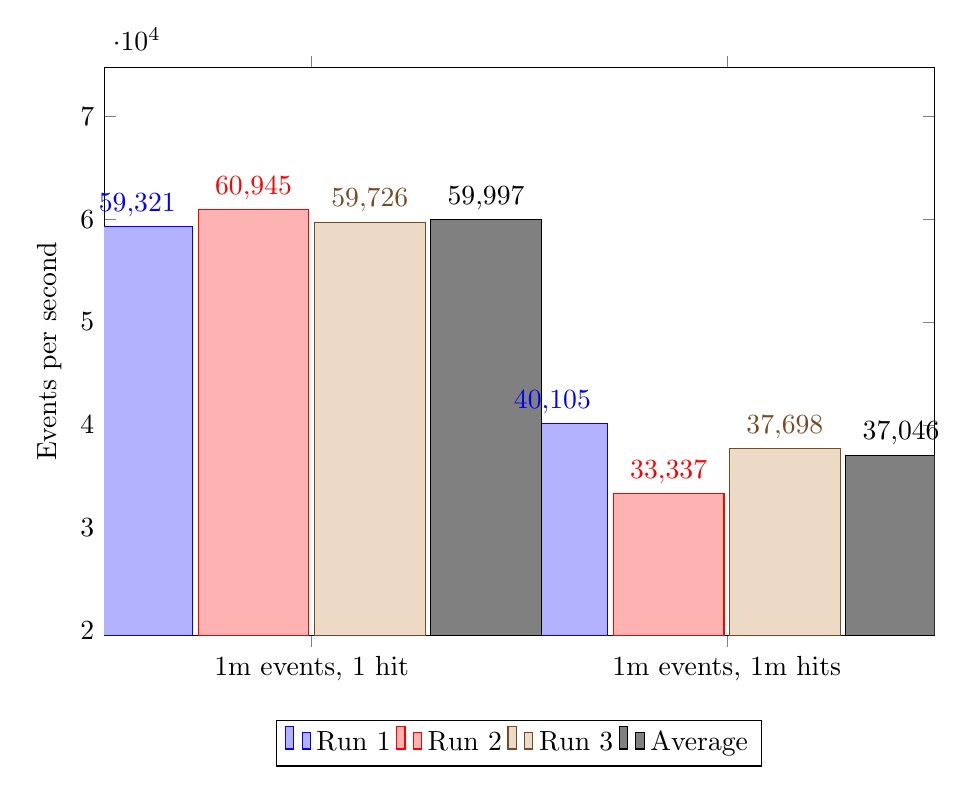
\begin{tikzpicture}
\begin{axis}[
    xtick=data,
	height=250pt,
	ylabel=Events per second,
	enlargelimits=0.5,
	legend style={at={(0.5,-0.15)},
	anchor=north,legend columns=-1},
	ybar,
	bar width=40pt,
	symbolic x coords={{1m events, 1 hit}, {1m events, 1m hits}},
	nodes near coords,
	nodes near coords style={above}
]
\addplot coordinates {({1m events, 1 hit},59321) ({1m events, 1m hits},40105)};
\addplot coordinates {({1m events, 1 hit},60945) ({1m events, 1m hits},33337)};
\addplot coordinates {({1m events, 1 hit},59726) ({1m events, 1m hits},37698)};
\addplot coordinates {({1m events, 1 hit},59997) ({1m events, 1m hits},37046)}; 
\legend{Run 1, Run 2, Run 3, Average}
\end{axis}
\end{tikzpicture}
\caption{Comparing low signal high noise with high signal low noise datasets }
\label{fig:comparing-lshn-hsln}
\end{figure}
\chapter{Discussion}
\label{chap:discussion}

\section{Limitations of the study}
\label{sec:limitations}

\section{Future work}
\label{sec:futurework}

\todo{What could be expanded further upon in the future?}
\todo{Are there any experiments that we could have done, but didn't have the time to do? What could they tell us that we already didn't know?}
\chapter{Conclusion}
\label{chap:conclusion}
% ======== INSERT STUFF HERE ^^^ ========

\iffalse
\chapter{Definitions/Terms}
\label{chap:definitions}

\subsubsection{Context} -
\subsubsection{Context Engine} The part of the program that handles context.
\subsubsection{Event} A single Windows Event Log event.
\subsubsection{Goroutine} A lightweight thread handled by the Go runtime.
\subsubsection{Log line} A single line of a dataset, which consist of a single event.
\subsubsection{Sysmon} A Windows service and driver that uses XML configuration files to enhance the log data given by Windows Event Log.
\subsubsection{Windows Event Log} A built-in mechanism in Windows that logs telemetry of what happens on the system. Can be enhanced by installing and configuring Sysmon on the system.
\subsubsection{Worker} -

\chapter{Datasets}
\label{chap:datasets}

\section{Evaluation of existing datasets?}

\subsection{Boss of the SOC}
\todo{Describe the BOTS-datasets}
\todo{Run some actual tests against the dataset to see if we get a hit with our rules}

\subsubsection{Version 1}
\url{https://github.com/splunk/botsv1}
\subsubsection{Version 2}
\url{https://github.com/splunk/botsv2}
\subsubsection{Version 3}
\url{https://github.com/splunk/botsv3}

\subsection{Mordor}
\url{https://github.com/hunters-forge/mordor}

\subsection{EVTX-ATTACK-SAMPLES}
\url{https://github.com/sbousseaden/EVTX-ATTACK-SAMPLES/}



\section{Mordor datasets}
The Mordor datasets are pre-recorded events generated by simulating adversarial techniques in a test environment using common red team tools like Empire and Cobalt Strike. The largest dataset in the collection aims to simulate a Advanced Persistent Threat (APT) known as APT3/Gothic Panda. The dataset contains two scenarios, both outlined in MITRE ATT\&CK Evaluation Operational Flow. The flow maps directly to MITREs ATT\&CK framework, by stepping through 10 different "steps".

\begin{enumerate}
\item Initial Compromise
\item Initial Discovery
\item Privilege Escalation
\item Discovery for Lateral Movement
\item Credential Access
\item Lateral Movement
\item Persistence
\item Collection
\item Exfiltration
\item Execution of Persistence
\end{enumerate}

The dataset contains approximately 100 000 log lines, and is made for security analysts to test their skills and tools using real known bad data.

\section{High signal, low noise dataset}
The concentrated dataset is a generated dataset that repeats the same 3 log lines that are enough to trigger a rule. The dataset is made in different sizes, from 1 000 lines, to 1 million lines.

This dataset is in no way "realistic", and is only used for performance testing when evaluating our real-time analysis throughput in a "worst case"-scenario setting.

\section{Low signal, high noise dataset}
This is the opposite of the highly concentrated dataset which contained the necessary log lines to repeatedly trigger a specific rule. This dataset only contains the nessessary events to trigger a single rule once, the rest of the events are simply background noise.

\section{Baseline dataset}
This dataset is a dataset with events that are all benign. This dataset is useful for measuring the speed at which the tools process and analyse the events, without triggering any rules.

\section{Dataset discussion}

\subsection{Are they realistic?}


\subsection{Are they representative?}
\subsubsection{Concentrated dataset}
The concentrated dataset is used strictly for measuring the performance of the systems in a worst-case scenario, and the dataset is in itself not representative of a real world scenario, ingesting log data that doesn't contain malice.

\subsubsection{Mordor datasets}
The Mordor datasets are not as concentrated and gathered from a test environment using realistic tools, techniques and procedures based on the MITRE ATT\&CK framework.



\chapter{Experiments}
\label{chap:experiments}

- Created a program that can parse log data in real time, and do correlation on the data..
- Implemented several versions that


Simple Event Correlator (SEC).
\section{Terminology}
\subsection{Context}
\subsubsection{Context Engine}

The context engine is 

\subsection{Worker}

A worker is a Goroutine that has the sole job of reading an event from a channel, trying to match the event to the given set of rules. If there is a match, the worker will decide if it has to 

\subsubsection{Goroutines}

A Goroutine is a lightweight thread that is managed by the Go runtime. it is not a thread in the traditional sense.


\section{Created a implementation that uses Simple Event Correlators own rule format (regex based)}

\subsection{SEC rule format}



\begin{lstlisting}
type=single
ptype=regexp
pattern=(\S+)sshd.*
desc=This is a description
\end{lstlisting}

\subsubsection{type}
Type of rule. There are many different types here.
I have focused on rules using "SingleWithThreshold" which takes an action if there are X number of matches in Y time.

Single

Suppress

Calendar

SingleWithSuppress

Pair

PairWithWindow

SingleWith2Thresholds

EventGroup

SingleWithScript

Jump

\subsubsection{ptype}
Pattern type. RegExp is a Perl regular expression. Can use variables.

SubStr

PerlFunc

Cached

TValue

\subsubsection{pattern}
The pattern that the log line will we tested against. The value of this pattern is based on the ptype. For example, if the ptype is set to "RegExp", the pattern will be a Perl regular expression.

\subsubsection{desc}
Description field. But used for defining "scopes" when correlating.

\subsubsection{action}
The action to take when the rule "hits".

\subsubsection{continue}

\subsubsection{context}

\subsection{Implementation}
As discussed in chapter X, the programming language Go was chosen for implementing our new program to analyze our datasets. I have chosen to only implement the SingleWithTreshold type, and the RegExp pattern type (ptype). The "SingleWithTreshold" type triggers an action if there are X number of matches within Y time. We consider this to be the most usable rule type for our purpose. For the pattern type, we choose to use "RegExp", which are Perl regular expressions. We consider this to be the best option for matching against syslog-based log lines.

Other than the fact that Go is a compiled language and Perl is a interpreted language, the main additions in our implementation is that our version:
\begin{itemize}
    \item Uses Go channels for re-injecting events into the context engine.
    \item The use of channels and goroutines gives us the ability to run in a threaded matter, utilizing multiple cores.
\end{itemize}

\subsubsection{Workers}
\todo{What are workers?}

\subsection{Results}
We want to see if our Go implementation can out-perform SEC when handling a high signal, low noise dataset. The following table shows the results for that:
\\
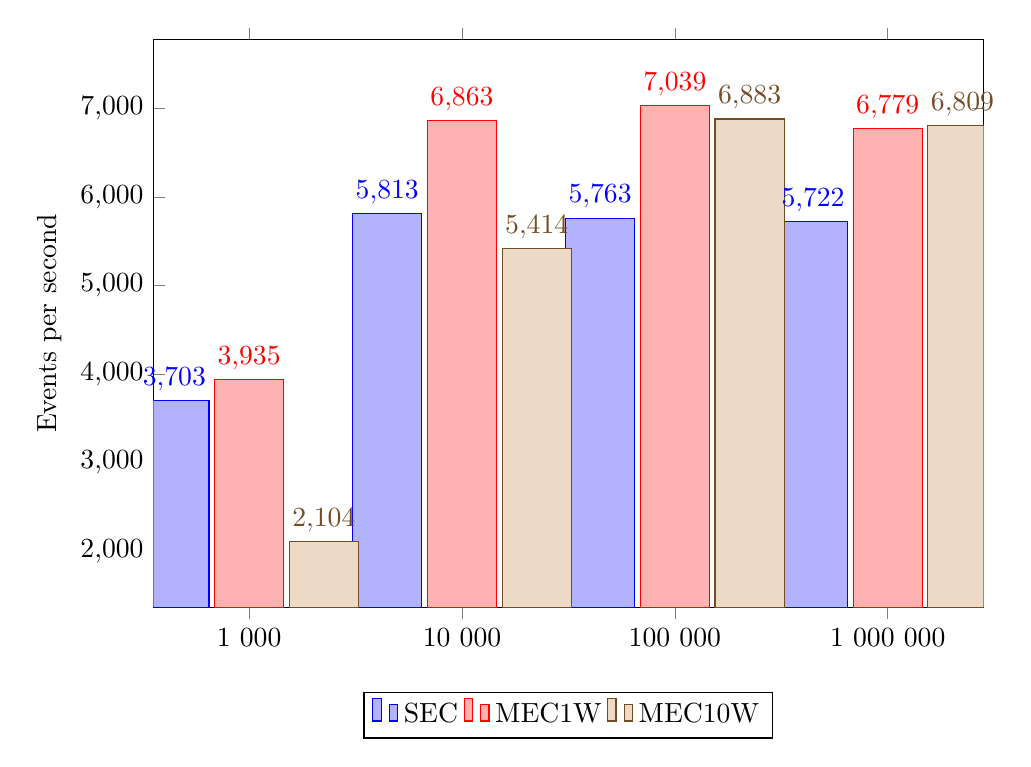
\begin{tikzpicture}
\begin{axis}[
    xtick=data,
	height=250pt,
	ylabel=Events per second,
	enlargelimits=0.15,
	legend style={at={(0.5,-0.15)},
	anchor=north,legend columns=-1},
	ybar,
	bar width=25pt,
	symbolic x coords={1 000, 10 000, 100 000, 1 000 000},
	nodes near coords,
	nodes near coords style={above}
]
\addplot coordinates {(1 000,3703) (10 000,5813) (100 000,5763) (1 000 000,5722)}; % SEC
\addplot coordinates {(1 000,3935) (10 000,6863) (100 000,7039) (1 000 000,6779)}; % MEC1W
\addplot coordinates {(1 000,2104) (10 000,5414) (100 000,6883) (1 000 000,6809)}; % MEC10W
\legend{SEC, MEC1W, MEC10W}
\end{axis}
\end{tikzpicture}
\\
These tests are run with 1 logical core on a "Intel(R) Core(TM) i7-7600U CPU @ 2.80GHz" (2 cores x 2 threads per core = max 4 logocal cores) and 24GB RAM.

\begin{itemize}
    \item Why is the MEC10W slower?
    \item Why are the runs on the 1 000 dataset generally lower?
\end{itemize}

By using all CPU cores available (4) instead of a single one, we can take better advantage of Gos concurrency model, and raise the throughput when using multiple workers and CPUs:

\pgfplotsset{scaled y ticks=false}
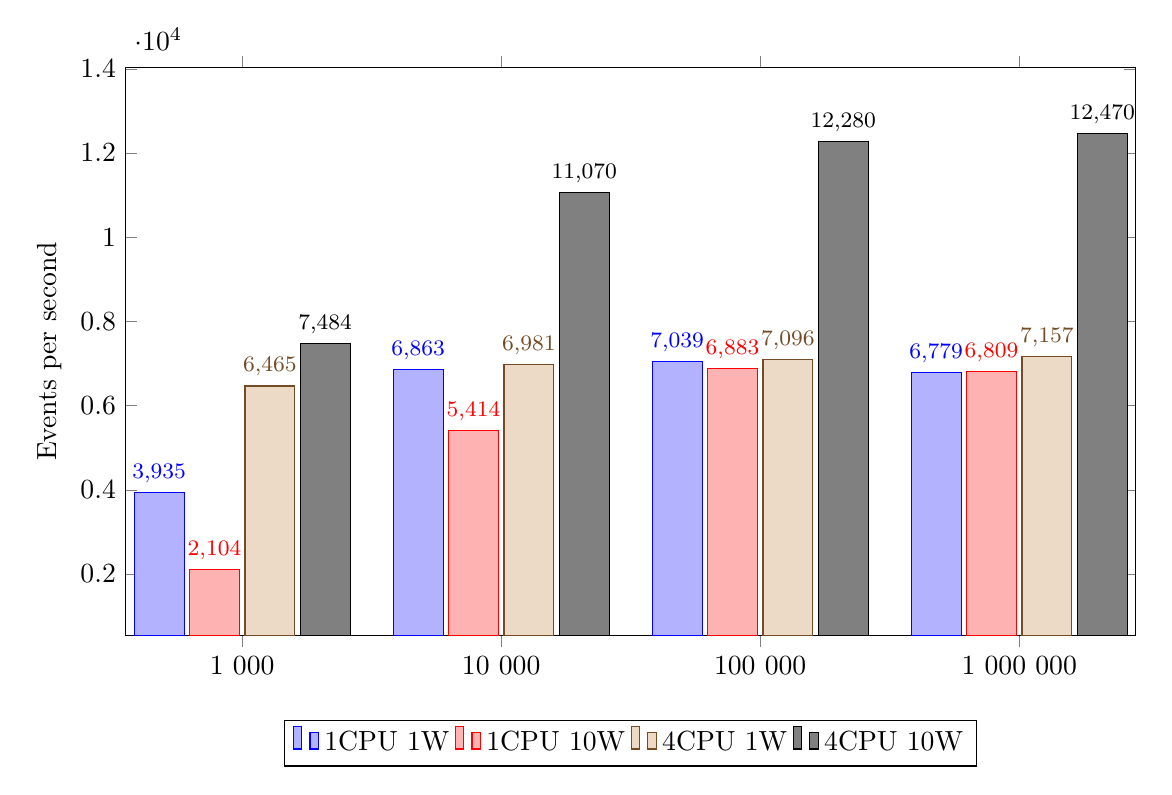
\begin{tikzpicture}
\begin{axis}[
    xtick=data,
    width=410pt,
	height=250pt,
	ylabel=Events per second,
	enlargelimits=0.15,
	legend style={at={(0.5,-0.15)},
	anchor=north,legend columns=-1},
	ybar,
	bar width=18pt,
	symbolic x coords={1 000, 10 000, 100 000, 1 000 000},
	nodes near coords,
	nodes near coords style={above, font=\footnotesize},
]
\addplot coordinates {(1 000,3935) (10 000,6863) (100 000,7039) (1 000 000,6779)}; % 1CPU 1W
\addplot coordinates {(1 000,2104) (10 000,5414) (100 000,6883) (1 000 000,6809)}; % 1CPU 10W
\addplot coordinates {(1 000,6465) (10 000,6981) (100 000,7096) (1 000 000,7157)}; % 4CPU 1W
\addplot coordinates {(1 000,7484) (10 000,11070) (100 000,12280) (1 000 000,12470)}; % 4CPU 10W
\legend{1CPU 1W , 1CPU 10W , 4CPU 1W , 4CPU 10W}
\end{axis}
\end{tikzpicture}

\begin{itemize}
\item Why is there a dip for 1CPU,10W when using a dataset of 1 000 events?
\item Why are the results of 1CPU,1W, 1CPU,10W and 10CPU,1W generally the same?
\item What can we say about 1CPU,10W "catching up" to the others around 100 000 events?
\end{itemize}

\section{Implemented a new rule format}
This format relies less on the extensive use of Regexes, as we saw in the rules used by Simple Event Correlator.

\subsection{Sigma}
\url{https://github.com/Neo23x0/sigma}

Sigma is an open standard for rules that are used to generically describe searches in log data. It is primarily used as a high-level rule that transcompile into SIEM queries like Splunk, ElasticSearch, QRadar, etc.

The rules are written in YAML (Yet Another Markup Language), and are key-value based.

\com{Testing}
\todo{Do somethiing}
\n{Testing note}
\begin{lstlisting}
title: Quick Execution of a Series of Suspicious Commands
id: 61ab5496-748e-4818-a92f-de78e20fe7f2
description: Detects multiple suspicious process in a limited timeframe
status: experimental
references:
    - https://car.mitre.org/wiki/CAR-2013-04-002
    - https://car.mitre.org/wiki/CAR-2013-04-003
author: juju4
modified: 2012/12/11
tags:
    - car.2013-04-002
logsource:
    category: process_creation
    product: windows
detection:
    selection:
        CommandLine:
            - ipconfig
            - arp
            - echo
    timeframe: 10s
    condition: selection | count() by MachineName > 3
falsepositives:
    - False positives depend on scripts and administrative tools used in the monitored environment
level: low
\end{lstlisting}

\subsection{Context}
\todo{What is context?}

\subsection{The Context Engine}
We are using a shared map between the "workers" of the application.

\subsection{Results}

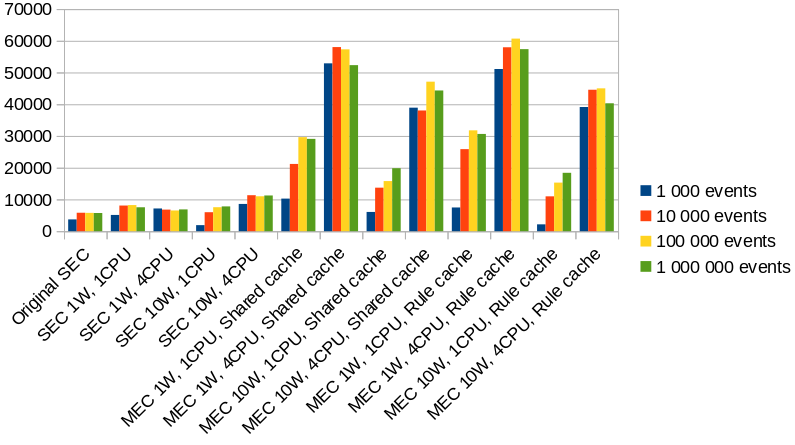
\includegraphics[scale=0.525]{figures/new-rule-format/performance.png}
\\
Min hypotese her, er at ved å bruke flere regler som trenger kontekst, så vil vi få et enda større sprang mellom shared og rule-based caching enn det vi ser over.
\\
Under har jeg generert 1000 regler og kjørt MEC på disse. Høyere søyle er bedre. Det er ganske tydelig at event-per-sekund her faller drastisk, da det må itereres over flere regler (2 vs 1000).
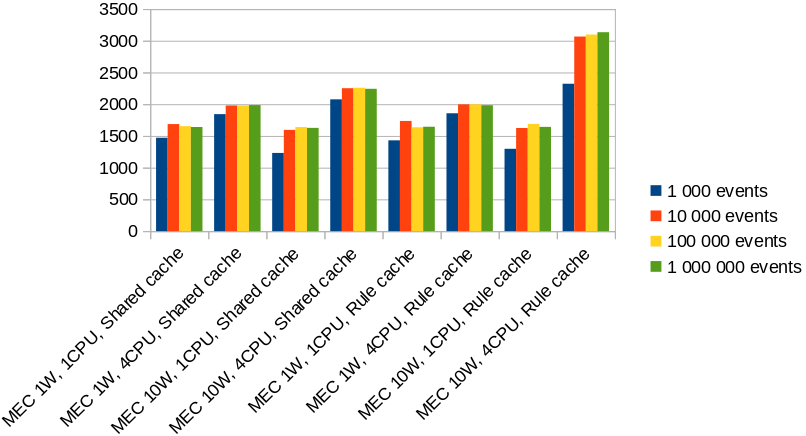
\includegraphics[scale=0.525]{figures/new-rule-format/performance-2.png}
\\
Som forventet så ser vi at rule-cache med 10W og 4CPU gir en 39.77\% økning sett opp imot 10W og 4CPU og shared caching.

Det som er interessant her er at det er liten forskjell mellom (1W, 1CPU), (10W, 1CPU) og (1W, 4CPU) mellom de forskjellige cache-typene. Dette gir mening, da lavt antall workers og CPU ikke drar ordentlig nytte av rule-based caching, og vil da falle ned til samme hastighet som shared cache.
\chapter{Introduction}
\label{chap:introduction}

\iffalse
Scrutiny of the introduction - http://sepwww.stanford.edu/sep/prof/Intro.html
\fi

\iffalse
The review

Pick out about 3-10 papers providing a background to your research and say something about each of them. You could paraphrase a sentence or two from each abstract. The review is not intended to be a historical review going back to Newton or Descartes. Try to find a few papers by your office mates, your advisor, your predecessors, or other associates. That way you might find somebody to give you helpful criticism!

Anyone can follow these instructions and write a review that looks presentable. Where intelligence and skill are required is in organizing the review so that it leads up to something, namely, to your claim.
\fi

\iffalse
The claim

The most important part of the introduction is buried in the middle. It is the claim. The claim is where you claim your work is a worthwhile extension of the review you just wrote. If someone says your writing is "unmotivated," they are not insulting your humanity; it just means they can't find your claim.

In your claim you should use the personal pronoun "I" (or "we" if you aren't the sole author). The word "I" tells people where common knowledge runs out and your ideas begin. If you are writing a doctoral dissertation or an article for a refereed journal, then you should be making a new contribution to existing knowledge. Your paper is not acceptable without an identifiable claim.
\fi

\iffalse
I believe that by using a more modern pipeline, programming language and ruleset for event correlation, we can improve not just the correlation throughput (events per second), but also make it simpler for security analysts to create, edit and manage correlation rules.
\fi

\iffalse
The agenda

An agenda is found at the end of many introductions. It summarizes what you will show the reader as your paper progresses. Your agenda will be dull if it is merely a recital of the topics you will cover. Your agenda should tell how your paper works to fulfill your claim. In this way your agenda should clarify your claim.

The agenda is not as important as the review and the claim. Keep it short.

Occasionally you will be fortunate enough to be writing about something in which some of your conclusions can be made in simple statements. If so, state them early, right after your agenda. You aren't trying to write a mystery! Many more people will begin reading your paper than will finish reading it. Motivate them to finish! Unfortunately, many technical papers do not lend themselves to early conclusions.
\fi
\iffalse
In this thesis, I will first give some background into the field of correlating event technologies, and give an overview of the state-of-the-art. Then I will explain the methods I have used to measure and analyze our results. After this, I will go into detail on our results, before we then discuss and analyse our results. Finally, I will conclude with some further work to be done.


\makebox[\linewidth]{\rule{\paperwidth}{0.4pt}}
\fi

This field is maturing, as focus has shifted from network monitoring and detection, to a more endpoint-centric approach....

\section{Problem description}
\label{sec:problemdescription}

We are seeing a movement away from network-based monitoring and detection. There are several reasons for this.

\begin{itemize}
    \item Increased usage of encrypted communications, as encryption has become standard and more popular than ever before. The continued introduction of other privacy-enhancing technologies like DNS-over-TLS/DNS-over-HTTPS will continue to hinder network-based monitoring and detection from being effective.
    \item Endpoints are no longer static inside a business network. Employees bring the computers with them outside of the office. Sometimes connected to their business' network via a Virtual Private Network (VPN), sometimes not.
    \item Network-based detection only give you a glimpse at what happens on the wire. There is not visibility into what is happening on the individual endpoints connected to the network.
\end{itemize}
The trend seems to be moving more towards host-based monitoring and detection instead. Traditionally, this has been frowned upon, as CPU-intensive agents would have to be installed on the endpoints. But now we are seeing higher performing agents, as well endpoints with more performant hardware. There are several advantages to moving to endpoint monitoring and detection.

\begin{itemize}
    \item Host-based detection and response makes it easier to detect anomalies and badness using either 3rd party software, or built-in capabilities of the OS.
    \item We are not bound to a particular network for protection, so we are still covered monitoring and detection-wise when on the move.
    \item There is a constant development to allow further insight into what is happening on the endpoint by the OS-vendors.
\end{itemize}

Current detection analysis is based on aggregating log files into a centralized system known as a System Information and Event Management (SIEM) system. Traditionally in a SIEM, logs are analyzed after-the-fact. This has several drawbacks:

\begin{itemize}
    \item Security monitoring is reactive.
    \item Requires actively hunting for bad events.
\end{itemize}

Another huge problem with pure SIEM-based logging, as companies are collecting more and more logs, actively hunting for badness in those logs are becoming harder and more complex. I single log item from a single source is not enough to properly analyze what has happened in a system. Only by cross-correlating several log lines and log sources are we able fully understand the situation at hand.

An example of this might be that we have a log item X. This means Y and is not a indication of badness in and of itself.
But if we also see log item Y right before log item X, that could be a indication of attack-pattern X. Which is a known Indicator of Compromise.



\iffalse
FROM http://folk.uio.no/josang/papers/MJ2018-ICCSP.pdf
Current threat detection analysis approaches include aggregation of log files in a centralized system known as security information and event management (SIEM) which performs inspections
and flags anomalies. A SIEM system collects logs by deploying
multiple collection agents to gather security-related events from
end-user devices, servers, intrusion detection systems (IDS), intrusion prevention systems (IPS) and firewalls, network devices such as
routers and DNS servers and more. In particular, one resource that
has received considerable attention for endpoint visibility has been
Sysmon; a Windows system service and device driver that monitors
and logs system activity of Windows workstations. Approaches for
threat detection using Sysmon have been proposed mainly focusing
on search engines (NoSQL database systems) or graph databases.
\fi

\section{Justification, motivation and benefits}
\label{sec:justificationmotivationandbenefits}
...
There are several benefits of this approach. We are using more modern, industry-standard technology which improves scalability, availability and performance.

\section{Research questions}
\label{sec:researchquestions}

\begin{itemize}
\item How can we improve event correlation/the SEC algorithm...? Hvordan kan vi forbedre event log analyse?
Implementerer en mer effektiv versjon.
    \item How can we make event log analysis and correlation faster using a compiled programming language (Go) rather than a dynamic, interpreted language like Perl.
    \item How can we make event log correlation simpler for the analyst by utilizing a common alert format for writing and sharing rules, instead of the heavily regular expression-based apporach of SEC?
    \item How can we further improve the distributed nature of log ingestion and processing by using queuing technologies and a shared in-memory cache for context-information between the event analyzers.
    \item Does correlating events reduce the number of false positives, and therefore avoid "alert fatigue"?
\end{itemize}

\section{Planned contributions}
\label{sec:plannedcontributions}

This thesis will:

\begin{itemize}
    \item Implement and detail a system for correlating Windows Event Logs in near real time. Using Go.
    \item Analyze benefits and drawbacks of using our system versus other tools.
    \item Show how the system performs on real world data, with a focus on measures to reduce the number of false positives.
    \item Contribute rules for common attack techniques back to the community, that require correlation to avoid a high false-positive rate.
\end{itemize}


\section{Thesis Outline}
\label{sec:thesisoutline}

First, we will.... % includes latex files from the same directory
\chapter{Literature review}
\label{chap:literaturereview}

\chapter{Implementation}
\label{chap:implementation}
This has the description of how you actually went about implementing the project.  This should be focused on the interesting challenges and how those related to the project.

\todo{add more here}

\begin{figure}[h]  %t top, b bottom, p page | you can also use h to try to get the figure to appear at the current location
  \centering
  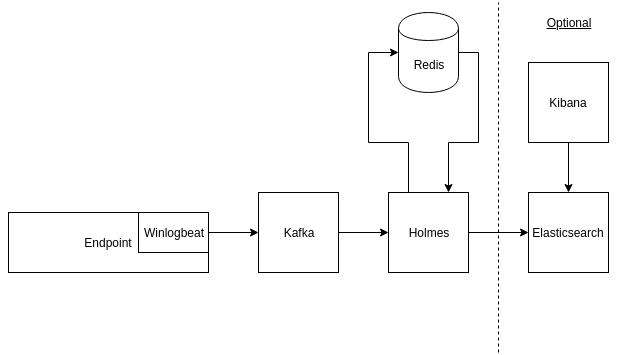
\includegraphics[width=.85\textwidth]{figures/holmes-architecture}
  \caption[An example figure.]{Minimal architecture. Every single node can be scaled both vertically and horizontally.}
  \label{fig:example}
\end{figure}

\include{inc/packages} % could be called Methodology or methods or any filename 
\include{inc/structure} % could be results
\chapter{Discussion}
\label{chap:discussion}

\section{Limitations of the study}
\label{sec:limitations}

\section{Future work}
\label{sec:futurework}

\todo{What could be expanded further upon in the future?}
\todo{Are there any experiments that we could have done, but didn't have the time to do? What could they tell us that we already didn't know?}
\chapter{Conclusion}
\label{chap:conclusion}
\fi
\ifthenelse{\boolean{HarvardCitations}}{%
	\bibliographystyle{agsm} % used for Harvard style references. Names - Humanities & Interaction Design
}{%
	\bibliographystyle{ntnuthesis/ntnuthesis} %used for Vancover style references. Numbers - Computer Science & Physics
}

\bibliography{thesis}

\appendix

\iffalse
\include{inc/rawdata}
\fi

\end{document}
